% =====================================================================
%  PeakCheck — Technical Supplement (English)
%  Compile: pdflatex -> bibtex -> pdflatex -> pdflatex
% =====================================================================
\documentclass[11pt,a4paper]{article}
\def\peakchecklang{english}
% =====================================================================
%  PeakCheck — shared LaTeX preamble
%  Used by:  Anleitung_PeakCheck.tex (DE), Manual_PeakCheck_EN.tex (EN),
%            Supplement_PeakCheck_EN.tex (EN)
%
%  Set the document language BEFORE % =====================================================================
%  PeakCheck — shared LaTeX preamble
%  Used by:  Anleitung_PeakCheck.tex (DE), Manual_PeakCheck_EN.tex (EN),
%            Supplement_PeakCheck_EN.tex (EN)
%
%  Set the document language BEFORE % =====================================================================
%  PeakCheck — shared LaTeX preamble
%  Used by:  Anleitung_PeakCheck.tex (DE), Manual_PeakCheck_EN.tex (EN),
%            Supplement_PeakCheck_EN.tex (EN)
%
%  Set the document language BEFORE \input{preamble.tex}, e.g.
%      \def\peakchecklang{english}   % or:  \def\peakchecklang{ngerman}
%  Engine: pdflatex.  Bibliography: bibtex + natbib (plainnat).
% =====================================================================

\usepackage[T1]{fontenc}
\usepackage[utf8]{inputenc}
\providecommand{\peakchecklang}{english}
% Graceful fallback: if the requested German babel files are absent (minimal
% TeX Live), fall back to english so the file still compiles. A full TeX Live /
% Overleaf has texlive-lang-german, so there the document stays German.
\def\pklangde{ngerman}
\ifx\peakchecklang\pklangde
  \IfFileExists{ngermanb.ldf}{}{\def\peakchecklang{english}}
\fi
\usepackage[\peakchecklang]{babel}
\IfFileExists{lmodern.sty}{\usepackage{lmodern}}{}

\usepackage[a4paper,margin=2.3cm]{geometry}
\usepackage{amsmath}
\usepackage{amssymb}
\usepackage{mathtools}
\usepackage{graphicx}
\usepackage{xcolor}
\usepackage{listings}
\usepackage{booktabs}
\usepackage{array}
\usepackage{tabularx}
\usepackage{ragged2e}
\usepackage{enumitem}
\usepackage{caption}
\usepackage[numbers,sort&compress]{natbib}
\IfFileExists{microtype.sty}{\usepackage[protrusion=true,expansion=false]{microtype}}{}

% hyperref last
\usepackage[colorlinks=true,linkcolor=pkblue,citecolor=pkblue,urlcolor=pkblue]{hyperref}

% --- colours ---------------------------------------------------------
\definecolor{pkblue}{HTML}{1F4E79}
\definecolor{pkaccent}{HTML}{C55A11}
\definecolor{codebg}{HTML}{F4F6F8}
\definecolor{codeframe}{HTML}{D6DEE6}
\definecolor{kw}{HTML}{0B5394}
\definecolor{str}{HTML}{7F6000}
\definecolor{cmt}{HTML}{6A737D}
\definecolor{hdrgray}{HTML}{555555}

% --- captions --------------------------------------------------------
\captionsetup{font=small,labelfont=bf,labelsep=period}

% --- listings: Python -----------------------------------------------
\lstdefinestyle{py}{%
  language=Python,
  basicstyle=\ttfamily\footnotesize,
  keywordstyle=\color{kw}\bfseries,
  stringstyle=\color{str},
  commentstyle=\color{cmt}\itshape,
  numberstyle=\tiny\color{cmt},
  backgroundcolor=\color{codebg},
  frame=single,
  framerule=0.4pt,
  rulecolor=\color{codeframe},
  showstringspaces=false,
  breaklines=true,
  breakatwhitespace=true,
  columns=fullflexible,
  keepspaces=true,
  tabsize=4,
  xleftmargin=10pt,
  xrightmargin=4pt,
  aboveskip=2pt,
  belowskip=10pt,
}

% --- listings: TOML / console (generic, '#' comments) ---------------
\lstdefinestyle{conf}{%
  basicstyle=\ttfamily\footnotesize,
  keywordstyle=\color{kw},
  commentstyle=\color{cmt}\itshape,
  morecomment=[l]{\#},
  morestring=[b]",
  stringstyle=\color{str},
  backgroundcolor=\color{codebg},
  frame=single,
  framerule=0.4pt,
  rulecolor=\color{codeframe},
  showstringspaces=false,
  breaklines=true,
  columns=fullflexible,
  keepspaces=true,
  xleftmargin=10pt,
  xrightmargin=4pt,
  aboveskip=2pt,
  belowskip=10pt,
}

% --- helper macros ---------------------------------------------------
% inline monospace (detokenize so _, #, & etc. need no escaping)
\newcommand{\code}[1]{\texttt{\detokenize{#1}}}
% header line shown above a code listing: module path + function
\newcommand{\codehdr}[1]{\par\smallskip\noindent
  {\small\ttfamily\color{hdrgray}#1}\par\nobreak\vspace{1pt}}
% a "source / code reference" margin-style note inline
\newcommand{\srcref}[1]{\textnormal{\small\color{hdrgray}(#1)}}

% nicer default spacing for itemize
\setlist[itemize]{leftmargin=1.4em,topsep=2pt,itemsep=1pt}
\setlist[enumerate]{leftmargin=1.6em,topsep=2pt,itemsep=2pt}

% table helpers
\newcolumntype{L}{>{\RaggedRight\arraybackslash}X}
\renewcommand{\arraystretch}{1.15}

% section formatting (lightweight; optional package)
\IfFileExists{sectsty.sty}{\usepackage{sectsty}\allsectionsfont{\color{pkblue}}}{}

\setlength{\parskip}{0.4em}
\setlength{\parindent}{0pt}
, e.g.
%      \def\peakchecklang{english}   % or:  \def\peakchecklang{ngerman}
%  Engine: pdflatex.  Bibliography: bibtex + natbib (plainnat).
% =====================================================================

\usepackage[T1]{fontenc}
\usepackage[utf8]{inputenc}
\providecommand{\peakchecklang}{english}
% Graceful fallback: if the requested German babel files are absent (minimal
% TeX Live), fall back to english so the file still compiles. A full TeX Live /
% Overleaf has texlive-lang-german, so there the document stays German.
\def\pklangde{ngerman}
\ifx\peakchecklang\pklangde
  \IfFileExists{ngermanb.ldf}{}{\def\peakchecklang{english}}
\fi
\usepackage[\peakchecklang]{babel}
\IfFileExists{lmodern.sty}{\usepackage{lmodern}}{}

\usepackage[a4paper,margin=2.3cm]{geometry}
\usepackage{amsmath}
\usepackage{amssymb}
\usepackage{mathtools}
\usepackage{graphicx}
\usepackage{xcolor}
\usepackage{listings}
\usepackage{booktabs}
\usepackage{array}
\usepackage{tabularx}
\usepackage{ragged2e}
\usepackage{enumitem}
\usepackage{caption}
\usepackage[numbers,sort&compress]{natbib}
\IfFileExists{microtype.sty}{\usepackage[protrusion=true,expansion=false]{microtype}}{}

% hyperref last
\usepackage[colorlinks=true,linkcolor=pkblue,citecolor=pkblue,urlcolor=pkblue]{hyperref}

% --- colours ---------------------------------------------------------
\definecolor{pkblue}{HTML}{1F4E79}
\definecolor{pkaccent}{HTML}{C55A11}
\definecolor{codebg}{HTML}{F4F6F8}
\definecolor{codeframe}{HTML}{D6DEE6}
\definecolor{kw}{HTML}{0B5394}
\definecolor{str}{HTML}{7F6000}
\definecolor{cmt}{HTML}{6A737D}
\definecolor{hdrgray}{HTML}{555555}

% --- captions --------------------------------------------------------
\captionsetup{font=small,labelfont=bf,labelsep=period}

% --- listings: Python -----------------------------------------------
\lstdefinestyle{py}{%
  language=Python,
  basicstyle=\ttfamily\footnotesize,
  keywordstyle=\color{kw}\bfseries,
  stringstyle=\color{str},
  commentstyle=\color{cmt}\itshape,
  numberstyle=\tiny\color{cmt},
  backgroundcolor=\color{codebg},
  frame=single,
  framerule=0.4pt,
  rulecolor=\color{codeframe},
  showstringspaces=false,
  breaklines=true,
  breakatwhitespace=true,
  columns=fullflexible,
  keepspaces=true,
  tabsize=4,
  xleftmargin=10pt,
  xrightmargin=4pt,
  aboveskip=2pt,
  belowskip=10pt,
}

% --- listings: TOML / console (generic, '#' comments) ---------------
\lstdefinestyle{conf}{%
  basicstyle=\ttfamily\footnotesize,
  keywordstyle=\color{kw},
  commentstyle=\color{cmt}\itshape,
  morecomment=[l]{\#},
  morestring=[b]",
  stringstyle=\color{str},
  backgroundcolor=\color{codebg},
  frame=single,
  framerule=0.4pt,
  rulecolor=\color{codeframe},
  showstringspaces=false,
  breaklines=true,
  columns=fullflexible,
  keepspaces=true,
  xleftmargin=10pt,
  xrightmargin=4pt,
  aboveskip=2pt,
  belowskip=10pt,
}

% --- helper macros ---------------------------------------------------
% inline monospace (detokenize so _, #, & etc. need no escaping)
\newcommand{\code}[1]{\texttt{\detokenize{#1}}}
% header line shown above a code listing: module path + function
\newcommand{\codehdr}[1]{\par\smallskip\noindent
  {\small\ttfamily\color{hdrgray}#1}\par\nobreak\vspace{1pt}}
% a "source / code reference" margin-style note inline
\newcommand{\srcref}[1]{\textnormal{\small\color{hdrgray}(#1)}}

% nicer default spacing for itemize
\setlist[itemize]{leftmargin=1.4em,topsep=2pt,itemsep=1pt}
\setlist[enumerate]{leftmargin=1.6em,topsep=2pt,itemsep=2pt}

% table helpers
\newcolumntype{L}{>{\RaggedRight\arraybackslash}X}
\renewcommand{\arraystretch}{1.15}

% section formatting (lightweight; optional package)
\IfFileExists{sectsty.sty}{\usepackage{sectsty}\allsectionsfont{\color{pkblue}}}{}

\setlength{\parskip}{0.4em}
\setlength{\parindent}{0pt}
, e.g.
%      \def\peakchecklang{english}   % or:  \def\peakchecklang{ngerman}
%  Engine: pdflatex.  Bibliography: bibtex + natbib (plainnat).
% =====================================================================

\usepackage[T1]{fontenc}
\usepackage[utf8]{inputenc}
\providecommand{\peakchecklang}{english}
% Graceful fallback: if the requested German babel files are absent (minimal
% TeX Live), fall back to english so the file still compiles. A full TeX Live /
% Overleaf has texlive-lang-german, so there the document stays German.
\def\pklangde{ngerman}
\ifx\peakchecklang\pklangde
  \IfFileExists{ngermanb.ldf}{}{\def\peakchecklang{english}}
\fi
\usepackage[\peakchecklang]{babel}
\IfFileExists{lmodern.sty}{\usepackage{lmodern}}{}

\usepackage[a4paper,margin=2.3cm]{geometry}
\usepackage{amsmath}
\usepackage{amssymb}
\usepackage{mathtools}
\usepackage{graphicx}
\usepackage{xcolor}
\usepackage{listings}
\usepackage{booktabs}
\usepackage{array}
\usepackage{tabularx}
\usepackage{ragged2e}
\usepackage{enumitem}
\usepackage{caption}
\usepackage[numbers,sort&compress]{natbib}
\IfFileExists{microtype.sty}{\usepackage[protrusion=true,expansion=false]{microtype}}{}

% hyperref last
\usepackage[colorlinks=true,linkcolor=pkblue,citecolor=pkblue,urlcolor=pkblue]{hyperref}

% --- colours ---------------------------------------------------------
\definecolor{pkblue}{HTML}{1F4E79}
\definecolor{pkaccent}{HTML}{C55A11}
\definecolor{codebg}{HTML}{F4F6F8}
\definecolor{codeframe}{HTML}{D6DEE6}
\definecolor{kw}{HTML}{0B5394}
\definecolor{str}{HTML}{7F6000}
\definecolor{cmt}{HTML}{6A737D}
\definecolor{hdrgray}{HTML}{555555}

% --- captions --------------------------------------------------------
\captionsetup{font=small,labelfont=bf,labelsep=period}

% --- listings: Python -----------------------------------------------
\lstdefinestyle{py}{%
  language=Python,
  basicstyle=\ttfamily\footnotesize,
  keywordstyle=\color{kw}\bfseries,
  stringstyle=\color{str},
  commentstyle=\color{cmt}\itshape,
  numberstyle=\tiny\color{cmt},
  backgroundcolor=\color{codebg},
  frame=single,
  framerule=0.4pt,
  rulecolor=\color{codeframe},
  showstringspaces=false,
  breaklines=true,
  breakatwhitespace=true,
  columns=fullflexible,
  keepspaces=true,
  tabsize=4,
  xleftmargin=10pt,
  xrightmargin=4pt,
  aboveskip=2pt,
  belowskip=10pt,
}

% --- listings: TOML / console (generic, '#' comments) ---------------
\lstdefinestyle{conf}{%
  basicstyle=\ttfamily\footnotesize,
  keywordstyle=\color{kw},
  commentstyle=\color{cmt}\itshape,
  morecomment=[l]{\#},
  morestring=[b]",
  stringstyle=\color{str},
  backgroundcolor=\color{codebg},
  frame=single,
  framerule=0.4pt,
  rulecolor=\color{codeframe},
  showstringspaces=false,
  breaklines=true,
  columns=fullflexible,
  keepspaces=true,
  xleftmargin=10pt,
  xrightmargin=4pt,
  aboveskip=2pt,
  belowskip=10pt,
}

% --- helper macros ---------------------------------------------------
% inline monospace (detokenize so _, #, & etc. need no escaping)
\newcommand{\code}[1]{\texttt{\detokenize{#1}}}
% header line shown above a code listing: module path + function
\newcommand{\codehdr}[1]{\par\smallskip\noindent
  {\small\ttfamily\color{hdrgray}#1}\par\nobreak\vspace{1pt}}
% a "source / code reference" margin-style note inline
\newcommand{\srcref}[1]{\textnormal{\small\color{hdrgray}(#1)}}

% nicer default spacing for itemize
\setlist[itemize]{leftmargin=1.4em,topsep=2pt,itemsep=1pt}
\setlist[enumerate]{leftmargin=1.6em,topsep=2pt,itemsep=2pt}

% table helpers
\newcolumntype{L}{>{\RaggedRight\arraybackslash}X}
\renewcommand{\arraystretch}{1.15}

% section formatting (lightweight; optional package)
\IfFileExists{sectsty.sty}{\usepackage{sectsty}\allsectionsfont{\color{pkblue}}}{}

\setlength{\parskip}{0.4em}
\setlength{\parindent}{0pt}


\title{\vspace{-1.5em}\color{pkblue}\bfseries PeakCheck --- Technical Supplement\\[2pt]
\normalsize\mdseries\color{black}Method, algorithms and annotated source code}
\author{Lukas Knauer \and Volker Sch\"unemann\\[-2pt]
{\small RPTU Kaiserslautern-Landau \textperiodcentered\ AG Sch\"unemann}}
\date{\small Version 1.0.0 \textperiodcentered\ MIT license \textperiodcentered\ 2026}

\hypersetup{
  pdftitle={PeakCheck -- Technical Supplement},
  pdfauthor={Lukas Knauer, Volker Schuenemann},
  pdfsubject={True-Voigt multi-peak fitting and peak-presence checking: method, algorithms and annotated source code},
  pdfkeywords={Voigt, Faddeeva, NNLS, peak fitting, baseline, spectroscopy, NRVS, NIS, PeakCheck}
}

\begin{document}
\maketitle
\thispagestyle{empty}

\noindent\fcolorbox{codeframe}{codebg}{%
\parbox{\dimexpr\linewidth-2\fboxsep\relax}{\small
This supplement derives every computational step of PeakCheck and shows the
corresponding excerpts of the \code{peakcheck} package --- closely following the
source, with brief inline comments added for orientation and longer passages
abbreviated by \code{...} --- each followed by a short explanation, so the code
can be followed directly. Every method is backed by a literature reference
(Section~19); the same references appear as NumPy-style docstrings in the source.
Code excerpts carry a header naming the exact submodule and function, e.g.\
\code{peakcheck/profiles.py --- voigt()}, so each formula can be located in the
source at a glance.}}

\medskip
{\small\tableofcontents}
\bigskip

% =====================================================================
\section{Overview and code map}
PeakCheck answers a single question: \emph{which peaks occur in the reference
data set, and which of them are present in the component data sets?} The flow is
linear and bundled in \code{run_analysis()}; the graphical interface
(\code{PeakCheckGUI}) and the batch mode (\code{run_headless()}) call the same
computational core.

\begin{figure}[h]
\centering
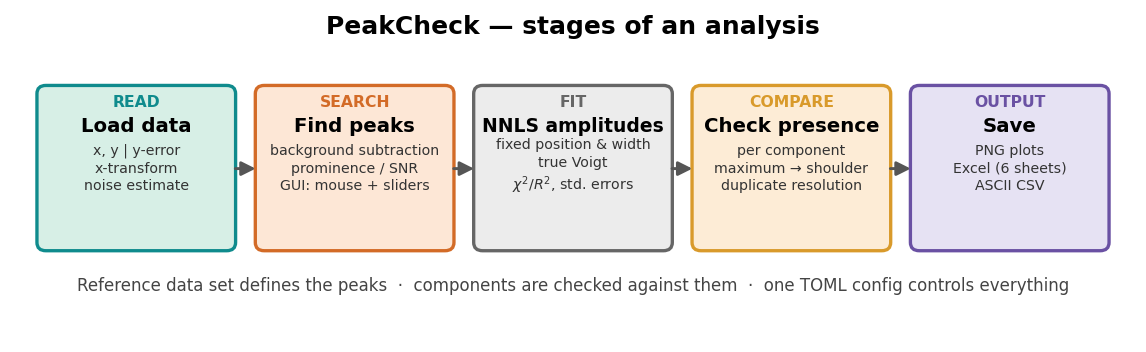
\includegraphics[width=0.92\linewidth]{figures/fig_pipeline.png}
\caption{The five stages of an analysis. The GUI and the headless run share the
same computational core.}
\end{figure}

\noindent The map below assigns the responsible functions to each stage; the
module table that follows names the submodule holding each function.

\begin{table}[h]\small\centering
\begin{tabularx}{\linewidth}{@{}l l L@{}}
\toprule
\textbf{Stage} & \textbf{Function(s)} & \textbf{Task}\\
\midrule
Read       & \code{load_xy}, \code{estimate_noise} & read the file robustly, transform $x$, estimate the noise\\
Profiles   & \code{voigt}, \code{gaussian}, \code{lorentzian}, \code{profile_shape} & area-normalised line shape\\
Background & \code{subtract_background} & remove the baseline as a rolling minimum\\
Search     & \code{search_peaks}, GUI \code{_on_click} & find peaks automatically / place them by mouse\\
Fit        & \code{fit_amplitudes}, \code{make_fit_mask}, \code{compute_model} & NNLS amplitudes at fixed positions/widths\\
Quality    & \code{fit_statistics} & $\chi^2$/$R^2$ and standard errors\\
Compare    & \code{check_peaks_in_component} & presence per component\\
Output     & \code{save_excel}, \code{save_csv}, \code{gather_parameters} & plots, Excel, ASCII CSV, metadata\\
\bottomrule
\end{tabularx}
\end{table}

\noindent The code is structured as a Python package --- each stage lives in its
own submodule, all sharing the same \code{Config} and feeding the same
\code{run_analysis()} core:

\begin{table}[h]\small\centering
\begin{tabularx}{\linewidth}{@{}l L@{}}
\toprule
\textbf{Module} & \textbf{Contents}\\
\midrule
\code{peakcheck.config}     & \code{Config}, \code{X_CONVERSIONS}, TOML I/O, axis transforms\\
\code{peakcheck.profiles}   & true Voigt, Gaussian, Lorentzian, \code{profile_shape}\\
\code{peakcheck.io}         & \code{load_xy}, \code{estimate_noise}\\
\code{peakcheck.background}  & \code{subtract_background}, \code{x_range_mask}\\
\code{peakcheck.fit}        & \code{search_peaks}, \code{make_fit_mask}, \code{fit_amplitudes}, \code{fit_statistics}\\
\code{peakcheck.presence}   & \code{check_peaks_in_component}\\
\code{peakcheck.plots}      & \code{plot_fit_result}, \code{plot_component}, \code{_outpath}\\
\code{peakcheck.output}     & \code{gather_parameters}, \code{save_excel}, \code{save_csv}\\
\code{peakcheck.pipeline}   & \code{run_analysis}, \code{run_headless}, \code{find_component_files}\\
\code{peakcheck.gui}        & \code{PeakCheckGUI} (Tkinter)\\
\code{peakcheck.cli}        & CLI: \code{main}, \code{build_arg_parser}\\
\bottomrule
\end{tabularx}
\end{table}

\noindent The public surface is re-exported from \code{peakcheck/__init__.py}, so
\code{from peakcheck import voigt, fit_amplitudes, run_analysis} keeps working.
The \code{peakcheck.py} file at the project root is a thin launcher that forwards
to the package.

% =====================================================================
\section{Configuration (Config / TOML)}
All parameters live in a \code{@dataclass} \code{Config} with defaults and helper
methods. The widths \code{wg} (Gaussian FWHM) and \code{wl} (Lorentzian FWHM) are
turned into the profile parameters by \code{sigma()} and \code{gamma()}:
\[
\sigma = \frac{f_G}{2\sqrt{2\ln 2}}\ \ \srcref{\code{sigma()}},
\qquad
\gamma = \frac{f_L}{2}\ \ \srcref{\code{gamma()}}.
\]

\codehdr{peakcheck/config.py --- Config.effective\_fwhm() (total FWHM of the Voigt profile)}
\begin{lstlisting}[style=py]
def effective_fwhm(self) -> float:
    p = str(self.profile).lower()
    if p in ("gauss", "gaussian"):
        return self.wg
    if p in ("lorentz", "lorentzian"):
        return self.wl
    return 0.5346 * self.wl + np.sqrt(0.2166 * self.wl ** 2 + self.wg ** 2)
\end{lstlisting}

\noindent The Voigt FWHM has no closed form; the empirical approximation of
Olivero \& Longbothum~\citep{Olivero1977} (accurate to about $0.02\,\%$) is used.
\code{load_config()} reads the TOML file section by section and flattens the
tables into the flat \code{Config}; \code{write_template()} writes a commented
template. Since TOML has no \code{null}, empty strings for \code{x_min}/\code{x_max}
are turned back into \code{None} by \code{_coerce_nullable()} (Section~18).

\smallskip
\noindent\textit{Because the GUI, the headless run and the TOML all build on the
same \code{Config}, a given parameter set always yields the same result,
independent of the entry path --- the basis of reproducibility (Section~11).}

% =====================================================================
\section{Reading and noise estimation}
\code{load_xy()} reads text files with two or three columns. A fast path
(\code{numpy.loadtxt}) is tried first; on failure a tolerant line-by-line parser
takes over, coping with header lines, comment characters (\code{# ! \%}), comma
decimal separators and extra columns. The file extension does not matter
(\code{.dat}, \code{.txt}, \code{.csv}, \code{.xy}, \code{.asc}, \code{.tsv},
\code{.prn}, \code{.nis}, \dots); values may be separated by whitespace, tabs,
commas or semicolons. A German-style decimal comma is distinguished from a
separator comma by anchoring on the whitespace-token count: if every
whitespace-separated token is a number once its comma is read as a decimal point,
the commas are decimal points; otherwise they are field separators (so
\code{10,5 100,2} reads as two values while \code{1,2,3} reads as three). Non-finite rows are dropped, the data are
sorted by ascending $x$, and the transform is applied (affine or reciprocal,
Section~3.1). Files ending in \code{.fio} (DESY/PETRA-III format) take a separate
path that parses the \code{\%d} data block and its \code{Col} declarations and
selects the $x$/$y$ columns via \code{fio_x_column}/\code{fio_y_column}; the
result then follows the same transform, sorting and noise handling. The third
column is optional (\code{error_column}); if it is absent,
\code{estimate_noise()} estimates a constant noise robustly from the first
differences:

\codehdr{peakcheck/io.py --- estimate\_noise() (robust noise estimate without an error column)}
\begin{lstlisting}[style=py]
def estimate_noise(y):
    d = np.diff(np.asarray(y, dtype=float))
    if len(d) == 0:
        return 1.0
    mad = np.median(np.abs(d - np.median(d)))
    sigma = 1.4826 * mad / np.sqrt(2.0)
    if not np.isfinite(sigma) or sigma <= 0:
        sigma = np.std(y) if np.std(y) > 0 else 1.0
    return float(sigma)
\end{lstlisting}
\[
\sigma = 1.4826\cdot\frac{\operatorname{MAD}(\Delta y)}{\sqrt 2},
\qquad \Delta y_i = y_{i+1}-y_i.
\]
\begin{itemize}
\item \code{np.diff(y)} forms $\Delta y$; differencing suppresses smooth signal so
that only the high-frequency noise remains.
\item The factor $1.4826$ turns the MAD into a consistent estimator of the
standard deviation of normally distributed noise~\citep{RousseeuwCroux1993}.
\item $1/\sqrt 2$ corrects the variance doubling from differencing
($\operatorname{Var}(\Delta y)=2\sigma^2$).
\item The fallback to \code{std(y)}/$1.0$ guarantees a strictly positive $\sigma$
so the weighted fit never divides by zero.
\end{itemize}
The return flag \code{had_errors} records whether real errors were present --- it
drives the error interpretation in Section~8.

\subsection{Axis transform: affine and reciprocal}
The $x$-axis is converted on load. \code{apply_x_transform()} supports two types
(with $a=$\code{x_scale}, $b=$\code{x_offset}):

\codehdr{peakcheck/config.py --- apply\_x\_transform() (affine and reciprocal conversion)}
\begin{lstlisting}[style=py]
def apply_x_transform(x, cfg):
    if str(cfg.x_transform).lower() == "reciprocal":
        x = np.asarray(x, dtype=float)
        safe = np.where(x == 0.0, np.nan, x)
        return cfg.x_scale / safe + cfg.x_offset
    return x * cfg.x_scale + cfg.x_offset
\end{lstlisting}
\[
\text{affine: } x' = a\,x + b,
\qquad
\text{reciprocal: } x' = \frac{a}{x} + b.
\]
\begin{itemize}
\item The affine form covers all linear unit changes, since energy, frequency and
wavenumber are proportional. NIS example: \code{x_scale}${}=8.065544$ converts
meV to $\mathrm{cm}^{-1}$.
\item The reciprocal form covers wavelength $\leftrightarrow$
wavenumber/energy/frequency, which are \emph{not} linear, e.g.\
$\tilde\nu\,[\mathrm{cm}^{-1}] = 10^{7}/\lambda\,[\mathrm{nm}]$. The line
\code{np.where(x==0, np.nan, x)} guards against division by zero.
\item A reciprocal map reverses the order, so \code{load_xy()} re-sorts by
ascending $x'$ afterwards.
\end{itemize}

Named presets live in the constant \code{X_CONVERSIONS} and are applied through
\code{apply_conversion()}, which sets factor, offset, transform type, axis label
and unit in one step:

\codehdr{peakcheck/config.py --- apply\_conversion() (apply a named preset)}
\begin{lstlisting}[style=py]
def apply_conversion(cfg, label) -> bool:
    if label not in X_CONVERSIONS:
        return False
    scale, offset, transform, xlabel, xunit = X_CONVERSIONS[label]
    cfg.x_scale, cfg.x_offset = scale, offset
    cfg.x_transform = transform
    cfg.x_label, cfg.x_unit = xlabel, xunit
    return True
\end{lstlisting}
The GUI shows only the affine presets; the reciprocal ones are reachable through
the TOML key \code{x_conversion} (e.g.\ \code{"nm -> eV (reciprocal)"}). Because
every other quantity (\code{x_min}, \code{x_max}, \code{wg}, \code{wl},
\code{tolerance}) is applied \emph{after} the transform, they always refer to the
target unit.

% =====================================================================
\section{Line profiles --- the true Voigt}
Each peak is an area-normalised profile (integral $1$); this makes the fitted
amplitude the integrated intensity directly and comparable across profiles.

\begin{figure}[h]
\centering
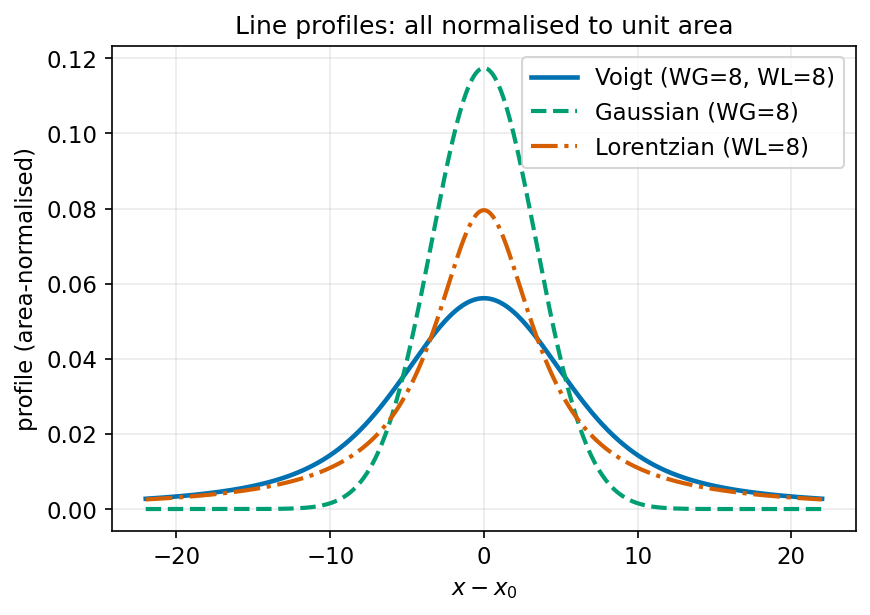
\includegraphics[width=0.78\linewidth]{figures/fig_profiles.png}
\caption{The three selectable profiles, each normalised to unit area.}
\end{figure}

The Voigt profile is the convolution of a Gaussian and a Lorentzian and is
computed \emph{exactly} through the Faddeeva function $w(z)$ --- not a
pseudo-Voigt:

\codehdr{peakcheck/profiles.py --- voigt() (exact Voigt via the Faddeeva function)}
\begin{lstlisting}[style=py]
def voigt(x, center, sigma, gamma):
    if sigma <= 0.0:
        return (gamma / np.pi) / ((x - center) ** 2 + gamma ** 2)
    z = ((x - center) + 1j * gamma) / (sigma * np.sqrt(2.0))
    return np.real(wofz(z)) / (sigma * np.sqrt(2.0 * np.pi))
\end{lstlisting}
\[
V(x) = \frac{\operatorname{Re}[w(z)]}{\sigma\sqrt{2\pi}},
\qquad
z = \frac{(x-x_0)+i\gamma}{\sigma\sqrt 2},
\qquad
w(z) = e^{-z^2}\operatorname{erfc}(-iz).
\]
\begin{itemize}
\item The special case \code{if sigma <= 0} returns the exact pure-Lorentzian
limit ($\sigma\to 0$); the pure-Gaussian limit ($\gamma\to 0$) is already
contained in $w(z)$.
\item \code{wofz} is the Faddeeva function from \code{scipy.special}~\citep{Virtanen2020};
for the definition see Abramowitz \& Stegun~\citep{AbramowitzStegun1972}, Sec.~7.1.
\item Dividing by $\sigma\sqrt{2\pi}$ normalises the area to $1$.
\end{itemize}

The pure shapes are dispatched by \code{profile_shape()} and are equally
area-normalised, so amplitudes stay comparable when the profile is switched:
\[
G(x) = \frac{1}{\sigma\sqrt{2\pi}}\exp\!\left[-\frac{(x-x_0)^2}{2\sigma^2}\right],
\qquad
L(x) = \frac{\gamma/\pi}{(x-x_0)^2+\gamma^2}.
\]

\codehdr{peakcheck/profiles.py --- gaussian(), lorentzian(), profile\_shape() (pure shapes + dispatch)}
\begin{lstlisting}[style=py]
def gaussian(x, center, sigma):
    return np.exp(-0.5 * ((x - center) / sigma) ** 2) / (sigma * np.sqrt(2.0 * np.pi))

def lorentzian(x, center, gamma):
    return (gamma / np.pi) / ((x - center) ** 2 + gamma ** 2)

def profile_shape(x, center, sigma, gamma, profile):
    p = str(profile).lower()
    if p in ("gauss", "gaussian"):
        return gaussian(x, center, sigma)
    if p in ("lorentz", "lorentzian"):
        return lorentzian(x, center, gamma)
    return voigt(x, center, sigma, gamma)
\end{lstlisting}

A pseudo-Voigt $\eta L + (1-\eta)G$ --- used by many programs --- gives a visibly
different curve:

\begin{figure}[h]
\centering
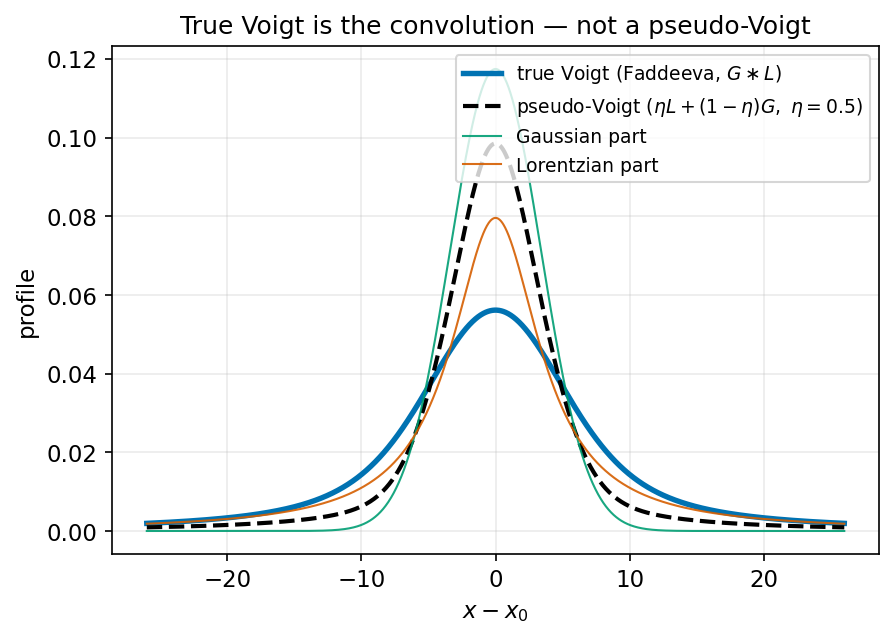
\includegraphics[width=0.74\linewidth]{figures/fig_voigt_true.png}
\caption{True Voigt (blue) versus pseudo-Voigt (red). PeakCheck uses the true
Voigt exclusively.}
\label{fig:voigttrue}
\end{figure}

\subsection{Why the Faddeeva function yields the Voigt}
The Voigt profile is, by definition, the convolution of a Gaussian line shape
(arising from inhomogeneous/instrumental broadening) with a Lorentzian (the
homogeneous, lifetime-broadened line),
\[
V(x) = (G \ast L)(x) = \int_{-\infty}^{\infty} G(x')\,L(x-x_0-x')\,\mathrm{d}x',
\]
with $G$ of standard deviation $\sigma$ and $L$ of half width at half maximum
$\gamma$, both centred and area-normalised. This integral has no elementary
closed form, but it is exactly the real part of the \emph{Faddeeva function}
$w(z) = e^{-z^2}\operatorname{erfc}(-iz)$ --- the scaled complex complementary
error function. Writing
\[
z = \frac{(x-x_0) + i\,\gamma}{\sigma\sqrt 2},
\qquad
V(x) = \frac{\operatorname{Re}\!\big[w(z)\big]}{\sigma\sqrt{2\pi}},
\]
collapses the convolution into a single special-function evaluation. This is
exact --- no series truncation and no pseudo-Voigt approximation --- and
numerically stable, because \code{scipy.special.wofz} evaluates $w(z)$ directly
to machine precision (quantified in Section~13). The two limiting cases follow
immediately from the same expression: as $\gamma\to 0$, $z$ becomes real and
$\operatorname{Re}[w(z)] = e^{-z^2}$, recovering the pure Gaussian; as
$\sigma\to 0$ (handled by the explicit branch in \code{voigt()}) the pure
Lorentzian remains. The widths of the two components,
\[
f_G = 2\sqrt{2\ln 2}\,\sigma, \qquad f_L = 2\gamma,
\]
do not simply add; the total Voigt FWHM is given to about $0.02\,\%$ by the
empirical approximation of Olivero \& Longbothum~\citep{Olivero1977}, which
\code{effective_fwhm()} uses (Section~2):
\[
f_V \approx 0.5346\,f_L + \sqrt{0.2166\,f_L^2 + f_G^2}.
\]
The equivalence is also evident numerically: a direct convolution of a sampled
Gaussian and Lorentzian reproduces the Faddeeva result to rounding
(Figure~\ref{fig:conv}).

\begin{figure}[h]
\centering
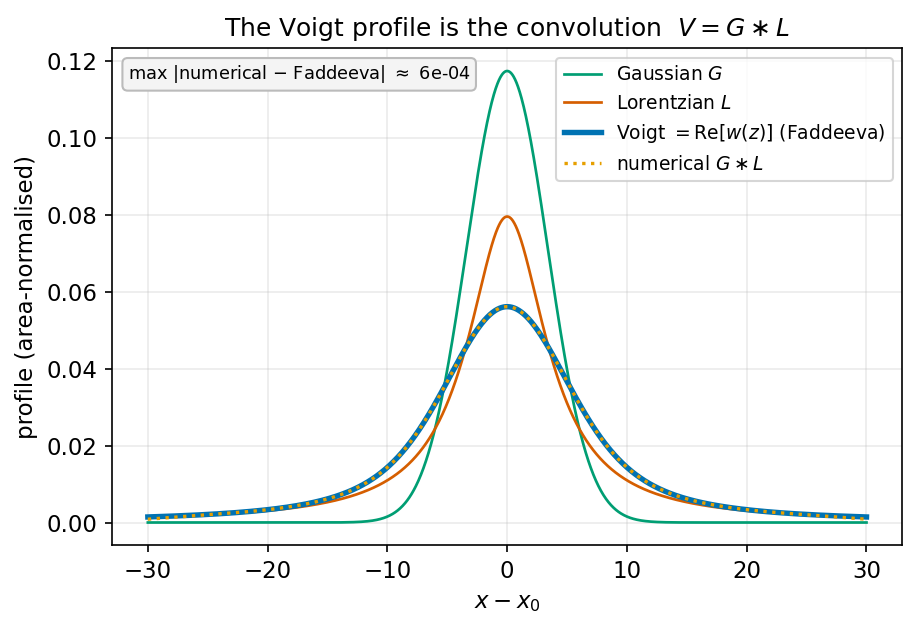
\includegraphics[width=0.78\linewidth]{figures/fig_convolution.png}
\caption{The Voigt profile (blue) \emph{is} the convolution of its Gaussian and
Lorentzian components; a direct numerical convolution (dotted) coincides with the
Faddeeva evaluation to the displayed tolerance --- it is the true Voigt, not a
pseudo-Voigt.}
\label{fig:conv}
\end{figure}

% =====================================================================
\section{Background subtraction}
Narrow peaks often sit on a broad pedestal. \code{subtract_background()}
estimates it as a rolling minimum and subtracts it:

\codehdr{peakcheck/background.py --- subtract\_background() (baseline as a rolling minimum)}
\begin{lstlisting}[style=py]
def subtract_background(y, window):
    if window <= 0:
        return y.copy()
    bg = minimum_filter1d(y, size=window, mode="reflect")
    return np.maximum(y - bg, 0.0)
\end{lstlisting}
\[
y_{\text{corr}}(i) = \max\!\Big(y(i) - \min_{|j-i|\le w/2} y(j),\ 0\Big).
\]
\begin{itemize}
\item \code{minimum_filter1d}~\citep{Virtanen2020} computes the rolling minimum
with window \code{window}; \code{mode="reflect"} handles the edges without
introducing spurious minima.
\item \code{np.maximum(..., 0.0)} prevents negative values after subtraction.
\item \code{window <= 0} disables the correction (returns a copy).
\end{itemize}

\begin{figure}[h]
\centering
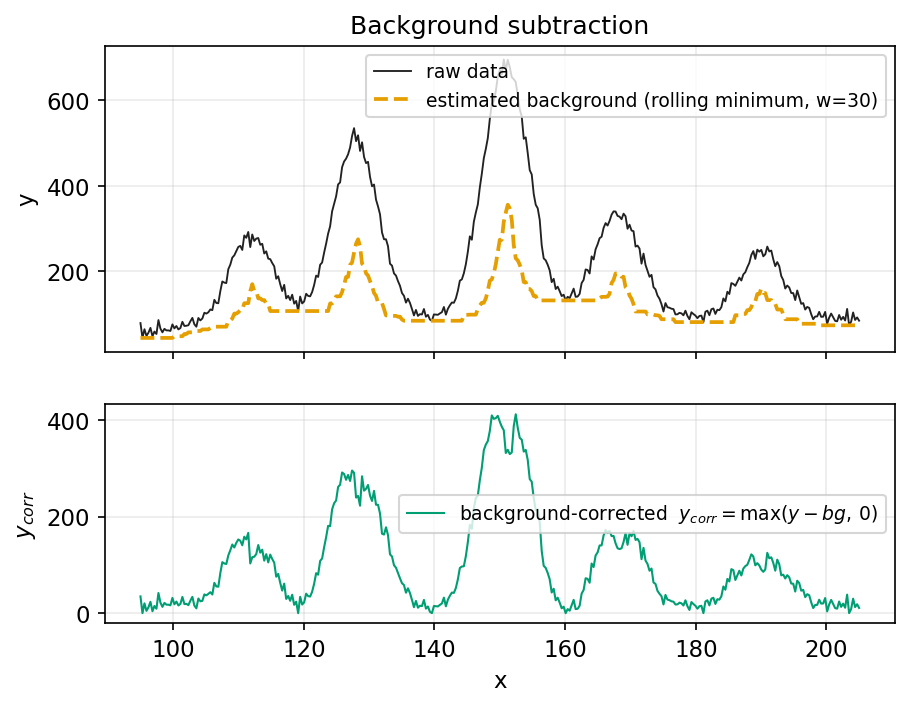
\includegraphics[width=0.80\linewidth]{figures/fig_background.png}
\caption{Top: raw data and the background estimated as a rolling minimum.
Bottom: the corrected signal.}
\end{figure}

The fit, the goodness-of-fit statistics, the component presence check and the
fit plot all operate on the same configured baseline, so the choice of baseline
never desynchronises the quantitative steps; the automatic search and the GUI
live preview use the rolling minimum as a candidate-detection aid.

\paragraph{Alternative baselines.} The rolling minimum is the default and is
robust for narrow peaks on a broad pedestal. Two smooth alternatives are
selectable through \code{baseline_method}: an iterative low-order polynomial
(\code{"polynomial"}, ModPoly style) and asymmetric least squares
(\code{"als"}, Eilers), the latter governed by a smoothness $\lambda$ and an
asymmetry weight $p$. Both estimate a smooth baseline that follows broad
structure while ignoring the peaks; the default reproduces all earlier results
exactly. Figure~\ref{fig:baselines} compares the three on one curved background.

\begin{figure}[h]\centering
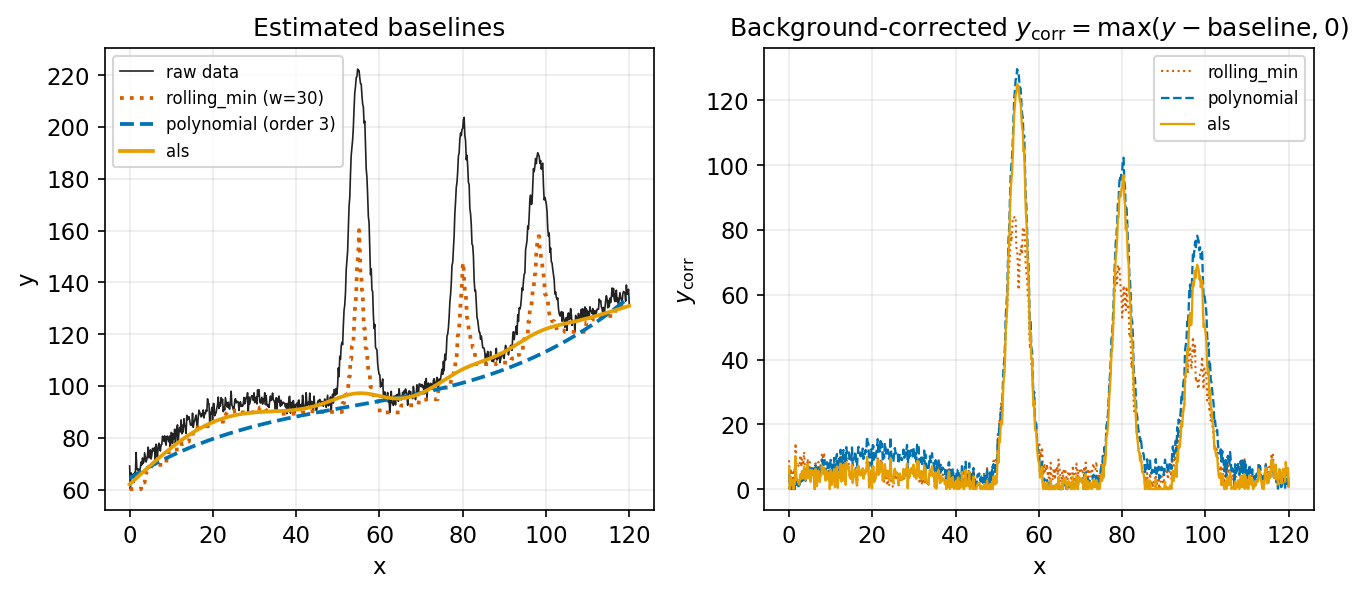
\includegraphics[width=0.96\linewidth]{figures/fig_baselines.png}
\caption{The three baseline estimators on the same curved, noisy background with
three peaks. Left: the estimated baselines --- the rolling minimum follows the
lower envelope in discrete steps, while the polynomial (ModPoly) and the
asymmetric-least-squares (ALS) curves are smooth. Right: the resulting corrected
signal $y_{\mathrm{corr}}=\max(y-\mathrm{baseline},0)$; ALS and the polynomial
flatten the inter-peak background more cleanly, whereas the rolling minimum leaves
a little residual structure. All three preserve the peak areas.}
\label{fig:baselines}
\end{figure}

% =====================================================================
\section{Peak search}
The automatic search works on the corrected data and filters by signal-to-noise
ratio:

\codehdr{peakcheck/fit.py --- search\_peaks() (automatic peak search with an SNR filter)}
\begin{lstlisting}[style=py]
def search_peaks(y, yerr, x, mask, prominence, distance, min_snr, bg_window):
    y_sub    = y[mask]
    yerr_sub = yerr[mask]
    y_corr   = subtract_background(y_sub, bg_window)

    local_idx, _ = find_peaks(y_corr, prominence=prominence,
                              distance=max(1, int(distance)))
    if min_snr > 0 and len(local_idx) > 0:
        snr = y_sub[local_idx] / yerr_sub[local_idx]
        local_idx = local_idx[snr >= min_snr]

    return np.where(mask)[0][local_idx]
\end{lstlisting}
\begin{itemize}
\item \code{subtract_background} first removes the baseline so that a sloping
background cannot hide weak peaks.
\item \code{find_peaks}~\citep{Virtanen2020} returns local maxima, filtered by
topographic \code{prominence} and a minimum \code{distance}.
\item The SNR filter $y_i/\sigma_i \ge \code{min_snr}$ is evaluated on the
\emph{raw} data so the threshold reflects the actual measured signal.
\item The return value maps the masked-region indices back to the full data set.
\end{itemize}
Thus a point counts as a peak (\emph{maximum}) only if it is a local maximum in
both the corrected and the raw data, stands out, and clears the SNR threshold. A
valley (lower than both neighbours) or a spurious peak merely lifted by the
subtraction is rejected.

\begin{figure}[h]
\centering
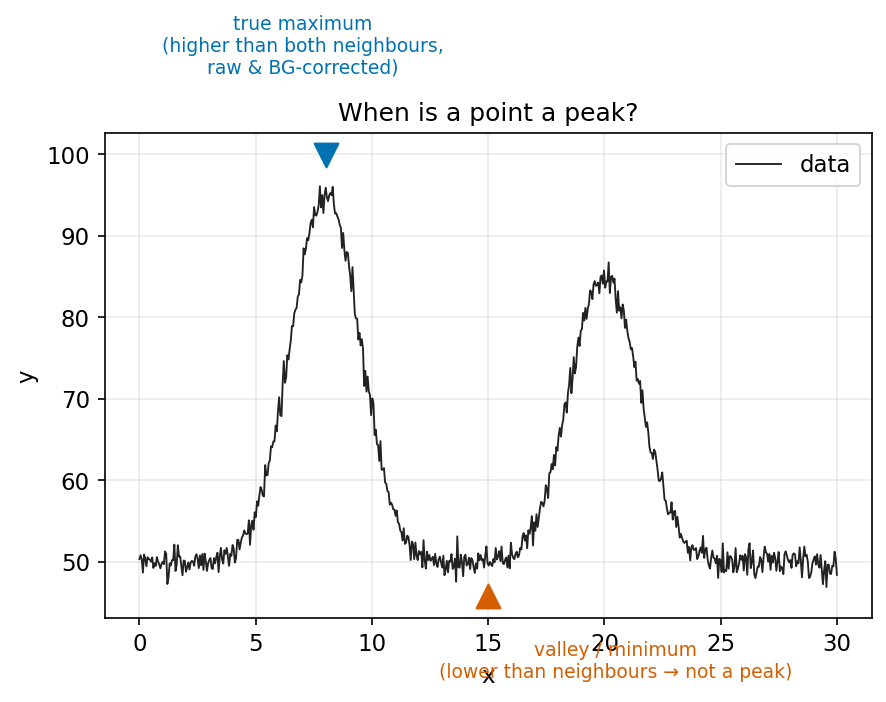
\includegraphics[width=0.72\linewidth]{figures/fig_peakcriteria.png}
\caption{True maximum (green) versus a valley (red).}
\end{figure}

% =====================================================================
\section{NNLS amplitude fit}
With fixed positions and widths the fit is linear in the amplitudes $A_k \ge 0$
and is solved as a weighted non-negative least-squares problem
(illustrated in Figure~\ref{fig:design}):

\codehdr{peakcheck/fit.py --- fit\_amplitudes() (weighted NNLS fit of the amplitudes)}
\begin{lstlisting}[style=py]
def fit_amplitudes(x, y, yerr, centers, cfg, fit_mask=None):
    if len(centers) == 0:
        return np.array([])
    sigma, gamma = cfg.sigma(), cfg.gamma()
    y_corr = subtract_background(y, cfg.bg_window)
    basis = np.column_stack(
        [profile_shape(x, c, sigma, gamma, cfg.profile) for c in centers])
    if fit_mask is None:
        fit_mask = np.ones(len(x), dtype=bool)
    W = 1.0 / yerr
    A = basis[fit_mask] * W[fit_mask, np.newaxis]
    b = (y_corr * W)[fit_mask]
    amplitudes, _ = nnls(A, b)
    return amplitudes
\end{lstlisting}
\[
\min_{\mathbf{A}\ge 0}\ \big\lVert W\,(B\mathbf{A}-\mathbf{y}_{\text{corr}})\big\rVert_2^2,
\qquad B_{ik} = P_k(x_i),\qquad W = \operatorname{diag}(1/\sigma_i).
\]
\begin{itemize}
\item The profile matrix \code{basis} holds one column $P_k(x_i)$ per peak
(\code{profile_shape} selects Voigt/Gaussian/Lorentzian).
\item $W = 1/\code{yerr}$ weights each point by the inverse uncertainty; \code{A}
and \code{b} are the weighted design matrix and target vector.
\item \code{fit_mask} restricts the fit to the window around the search range
(plus a tail margin, \code{make_fit_mask()}) so distant structure cannot bias the
amplitudes.
\item \code{scipy.optimize.nnls}~\citep{Virtanen2020} solves the problem with the
active-set algorithm of Lawson \& Hanson~\citep{LawsonHanson1995}; non-negativity
is physical (no negative intensities).
\item Because the profiles are area-normalised, $A_k$ is the integrated intensity
of the peak.
\end{itemize}

\begin{figure}[h]
\centering
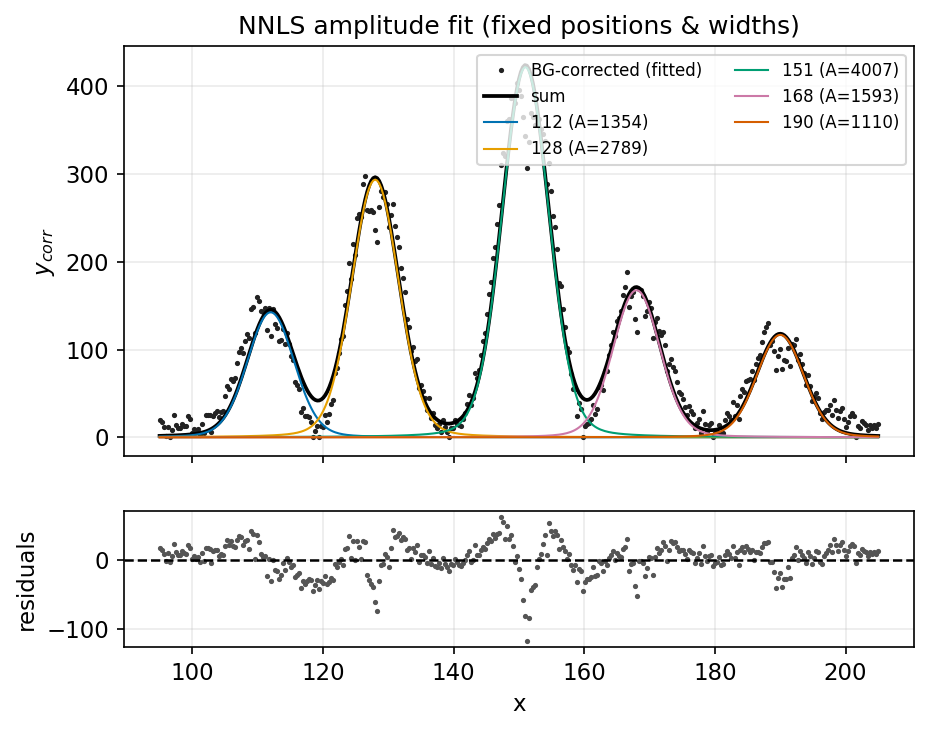
\includegraphics[width=0.82\linewidth]{figures/fig_fit.png}
\caption{NNLS fit: sum (red) and individual components over the corrected data,
with residuals below.}
\end{figure}

\begin{figure}[h]
\centering
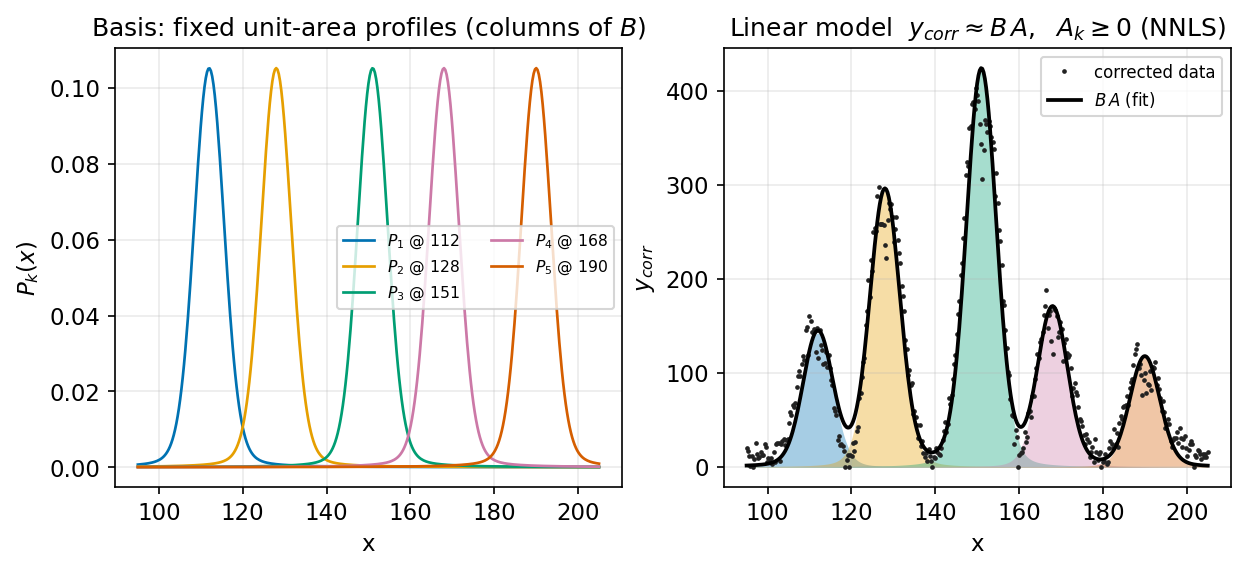
\includegraphics[width=0.96\linewidth]{figures/fig_design_matrix.png}
\caption{The amplitude fit is linear in the unknowns: the design matrix $B$ has
the fixed unit-area profiles as its columns (left), and the model is their
non-negative combination $B\,A$ (right). Only the heights $A_k$ are free, which
is what makes the problem a single convex NNLS solve.}
\label{fig:design}
\end{figure}

\subsection{Fit window and model assembly}
The fit runs not on the whole spectrum but on a window around the search range.
\code{make_fit_mask()} widens the range by $3(f_G+f_L)$ so the profile wings are
captured but distant structure cannot bias the amplitudes:

\codehdr{peakcheck/fit.py --- make\_fit\_mask() (fit window with a tail margin)}
\begin{lstlisting}[style=py]
def make_fit_mask(x, cfg):
    margin = 3.0 * (cfg.wg + cfg.wl)
    lo = (cfg.x_min - margin) if cfg.x_min is not None else x[0]
    hi = (cfg.x_max + margin) if cfg.x_max is not None else x[-1]
    return (x >= lo) & (x <= hi)
\end{lstlisting}

From the fitted amplitudes, \code{compute_model()} reassembles the sum and the
individual components --- the same routine produces the curves for the plot and
the Excel sheet:

\codehdr{peakcheck/fit.py --- compute\_model() (sum model from amplitudes)}
\begin{lstlisting}[style=py]
def compute_model(x, amplitudes, centers, sigma, gamma, profile):
    components = [amp * profile_shape(x, c, sigma, gamma, profile)
                  for amp, c in zip(amplitudes, centers)]
    total = np.sum(components, axis=0) if components else np.zeros_like(x)
    return total, components
\end{lstlisting}

\subsection{The active-set method (NNLS)}
The NNLS solver of Lawson \& Hanson~\citep{LawsonHanson1995} maintains a set of
``active'' peaks (amplitude $>0$) and a set pinned at the boundary ($A_k = 0$). It
iteratively tests whether admitting a pinned peak lowers the weighted sum of
squared residuals; otherwise the peak stays at zero. The result is the unique
minimum under the constraint $\mathbf{A}\ge 0$. For PeakCheck this means a peak
with no support in the data gets exactly $A_k = 0$ rather than a negative or noisy
small value --- physically correct, since negative intensities do not exist. This
very mechanism makes the fit robust against over-specified peaks.

% =====================================================================
\section{Goodness of fit and standard errors}
\code{fit_statistics()} assesses the fit and estimates the amplitude errors. The
core block:

\codehdr{peakcheck/fit.py --- fit\_statistics() (core block: $\chi^2$, covariance, error scaling)}
\begin{lstlisting}[style=py]
chi2     = float(np.sum((resid * w) ** 2))
n_active = int(np.sum(amplitudes > 0))
n_points = int(len(yf))
dof      = max(n_points - n_active, 1)
chi2_red = chi2 / dof

ss_res = float(np.sum(resid ** 2))
ss_tot = float(np.sum((yf - np.mean(yf)) ** 2))
r2     = 1.0 - ss_res / ss_tot if ss_tot > 0 else float("nan")

active = np.where(amplitudes > 0)[0]
stderr_stat = np.full(n, np.nan)
if len(active) > 0:
    Ba = Bf[:, active] * w[:, np.newaxis]      # weighted design matrix
    try:
        cov = np.linalg.inv(Ba.T @ Ba)         # (B^T W^2 B)^-1
        stderr_stat[active] = np.sqrt(np.clip(np.diag(cov), 0.0, None))
    except np.linalg.LinAlgError:
        pass

if eff_mode == "scaled":
    scale = np.sqrt(chi2_red) if np.isfinite(chi2_red) and chi2_red > 0 else 1.0
else:
    scale = 1.0
stderr = stderr_stat * scale
\end{lstlisting}
\[
\chi^2 = \sum_i\Big(\frac{r_i}{\sigma_i}\Big)^2,\quad
\chi^2_\nu = \frac{\chi^2}{N-N_{\text{active}}-N_{\text{extra}}},\quad
R^2 = 1 - \frac{\sum_i r_i^2}{\sum_i (y_i-\bar y)^2},\quad
\mathrm{Cov} = \big(B_{\text{act}}^{\top} W^2 B_{\text{act}}\big)^{-1}.
\]
Here $N_{\text{extra}}$ is the number of additional free parameters beyond the
amplitudes --- the refined positions and/or per-peak widths
(\code{n\_extra\_params} in \code{fit\_statistics}); it is $0$ in the default
fixed-position, fixed-width fit, so the formula reduces to the familiar
$\chi^2/(N-N_{\text{active}})$. When refinement is enabled these extra
parameters lower the degrees of freedom, so the reported $\chi^2_\nu$ accounts
for them honestly (see Section~15).
\begin{itemize}
\item The covariance is formed over the active set ($A_k > 0$) only;
\code{np.linalg.inv} gives $(B_{\text{act}}^{\top} W^2 B_{\text{act}})^{-1}$, whose
square-rooted diagonal are the statistical $1\sigma$
errors~\citep{BevingtonRobinson2003,Press2007}.
\item \code{np.clip(..., 0, None)} guards against slightly negative diagonal
values from rounding.
\item For peaks pinned at the boundary ($A_k = 0$) the error stays \code{NaN} ---
the linear covariance does not apply there.
\end{itemize}

\smallskip
\noindent\textbf{Two error modes --- and why the choice is physical.}
\begin{table}[h]\small\centering
\begin{tabularx}{\linewidth}{@{}l l L@{}}
\toprule
\textbf{Mode} & \textbf{Reported error} & \textbf{When correct}\\
\midrule
\code{statistical} & $\sigma_{A_k}$ (unscaled) &
when the error column is a genuine $1\sigma$ (e.g.\ photon counting / Poisson):
the random measurement error is reported honestly and $\chi^2_\nu$ stays a
separate model-adequacy diagnostic\\
\code{scaled} & $\sigma_{A_k}\cdot\sqrt{\chi^2_\nu}$ &
when the errors are only relative weights of unknown scale (the convention of
\code{curve_fit}, \code{absolute_sigma=False}~\citep{SciPyCurveFit})\\
\bottomrule
\end{tabularx}
\end{table}

\noindent\textit{Important:} with genuine measurement errors, $\chi^2_\nu > 1$
indicates \emph{systematic} model error (one fixed width for all peaks, an
approximate background, missing peaks) --- not larger noise. Folding that
systematic part into the random error bar via $\sqrt{\chi^2_\nu}$ would disguise a
model problem as a measurement uncertainty. When no genuine errors exist
(\code{had_errors=False}), \code{run_analysis()} switches to \code{scaled}
automatically via \code{force_scaled}, since the absolute noise scale is then
unknown.

% =====================================================================
\section{Presence check in the components}
For each reference peak, \code{check_peaks_in_component()} tests whether the
component has a peak within $\pm\,\code{tolerance}$. The search has three stages:
\begin{enumerate}
\item \textbf{Strict maximum.} A local maximum in both the corrected and the raw
data inside the (\code{EDGE_PAD}-extended) tolerance window; among several
candidates the one with the highest corrected intensity wins.
\item \textbf{Shoulder fallback.} If stage~1 finds nothing, inflection points of
$\mathrm{d}y/\mathrm{d}x$ (via \code{np.gradient}) are tested that reach at least
\code{SHOULDER_MIN_FRAC}${}=50\,\%$ of the window maximum and are not a valley.
\item \textbf{Duplicate resolution.} If two references claim the same point, the
closer one keeps it; the other searches for the next free maximum.
\end{enumerate}
A candidate is accepted only if its signal-to-noise ratio reaches
\code{snr_thresh} and $y_{\text{corr},i} > 0$. The SNR is evaluated by default on
the background-corrected signal, $y_{\text{corr},i}/\sigma_i$ --- the peak height
\emph{above} the background, which is the physically meaningful measure of
presence (the background itself is not a peak). Setting
\code{presence_baseline_corrected = false} reverts to the raw-signal ratio
$y_i/\sigma_i$. There is no re-fitting here --- only presence is determined.

\subsection{The three stages in code}
\textbf{Stage 1 --- strict maximum.} Within the (edge-padded) tolerance window,
local maxima of the corrected signal are located and accepted only if the point
is also a maximum of the raw data (this prevents a point merely lifted by the
background subtraction from passing as a peak). Among several candidates the one
with the highest corrected intensity wins:

\codehdr{peakcheck/presence.py --- check\_peaks\_in\_component(), stage 1}
\begin{lstlisting}[style=py]
# Step 1: strict local maximum in the (edge-padded) window
ext_peaks, _ = find_peaks(y_ext_corr)          # maxima of corrected signal
valid_ext = [ep for ep in ext_peaks
             if 0 < ep < len(y_ext_raw) - 1
             and y_ext_raw[ep] >= y_ext_raw[ep - 1]   # also a raw maximum
             and y_ext_raw[ep] >= y_ext_raw[ep + 1]
             and abs(x_sub[ext_idx_ar[ep]] - center) <= tolerance]
if len(valid_ext) > 0:
    best_ep = valid_ext[int(np.argmax(y_ext_corr[valid_ext]))]  # highest wins
    imax    = int(ext_idx_ar[best_ep])
\end{lstlisting}

\textbf{Stage 2 --- shoulder fallback.} If stage~1 finds nothing, inflection
points are sought via the derivative $\mathrm{d}y/\mathrm{d}x$ (with
\code{np.gradient}). A shoulder counts only if it reaches at least
\code{SHOULDER_MIN_FRAC}${}=50\,\%$ of the window maximum and is not a valley in
the raw data:

\codehdr{peakcheck/presence.py --- check\_peaks\_in\_component(), stage 2}
\begin{lstlisting}[style=py]
# Step 2: shoulder fallback (only if Step 1 found nothing)
if imax is None and len(window_idx) >= 3:
    dy = np.gradient(y_win_corr.astype(float))
    rising_cands,  _ = find_peaks(dy)         # inflection points of dy/dx
    falling_cands, _ = find_peaks(-dy)
    all_cands = np.concatenate([rising_cands, falling_cands])

    win_max_corr = np.max(y_win_corr)
    valid_shoulders = []
    for c in all_cands:
        if c == 0 or c == len(y_win_raw) - 1:
            continue
        if y_win_corr[c] < SHOULDER_MIN_FRAC * win_max_corr:    # >= 50 %
            continue
        if y_win_raw[c] < y_win_raw[c - 1] and y_win_raw[c] < y_win_raw[c + 1]:
            continue                                            # not a valley
        valid_shoulders.append(c)

    if len(valid_shoulders) > 0:
        shoulders_arr = np.array(valid_shoulders)
        best_local    = shoulders_arr[np.argmax(y_win_corr[shoulders_arr])]
        imax          = int(window_idx[best_local])
\end{lstlisting}

A located point is then accepted if it clears the SNR threshold --- on the signal
justified above (\code{y_snr} is corrected or raw):

\codehdr{peakcheck/presence.py --- check\_peaks\_in\_component(), acceptance}
\begin{lstlisting}[style=py]
snr   = y_snr[imax] / yerr_sub[imax]            # y_snr = corrected or raw
found = (snr >= snr_thresh) and (y_corr_sub[imax] > 0)
\end{lstlisting}

\textbf{Stage 3 --- duplicate resolution.} If two closely spaced references claim
the same data point, the nearer reference keeps it; the other searches for the
next free maximum in its own window (this prevents a single peak from being
counted twice):

\codehdr{peakcheck/presence.py --- check\_peaks\_in\_component(), stage 3}
\begin{lstlisting}[style=py]
# Step 3: duplicate resolution -- two references claim the same sample
j      = taken[imax_i]
dist_i = abs(x_sub[imax_i] - peak_centers[i])
dist_j = abs(x_sub[imax_i] - peak_centers[j])
winner, loser = (i, j) if dist_i <= dist_j else (j, i)   # nearer reference keeps it
taken[imax_i] = winner
# the loser searches the next free local maximum in its own window:
alt_peaks, _ = find_peaks(y_corr_sub[ext_l])
alt_valid = [ep for ep in alt_peaks
             if 0 < ep < len(ext_l) - 1
             and y_sub[ext_l[ep]] >= y_sub[ext_l[ep] - 1]
             and y_sub[ext_l[ep]] >= y_sub[ext_l[ep] + 1]
             and abs(x_sub[ext_l[ep]] - center_l) <= tolerance
             and int(ext_l[ep]) not in taken
             and int(ext_l[ep]) != imax_i]
\end{lstlisting}

This three-stage logic is deliberately conservative: it accepts only genuine
maxima or clear shoulders and resolves ambiguities geometrically (by proximity to
the reference position) rather than arbitrarily.

\begin{figure}[h]
\centering
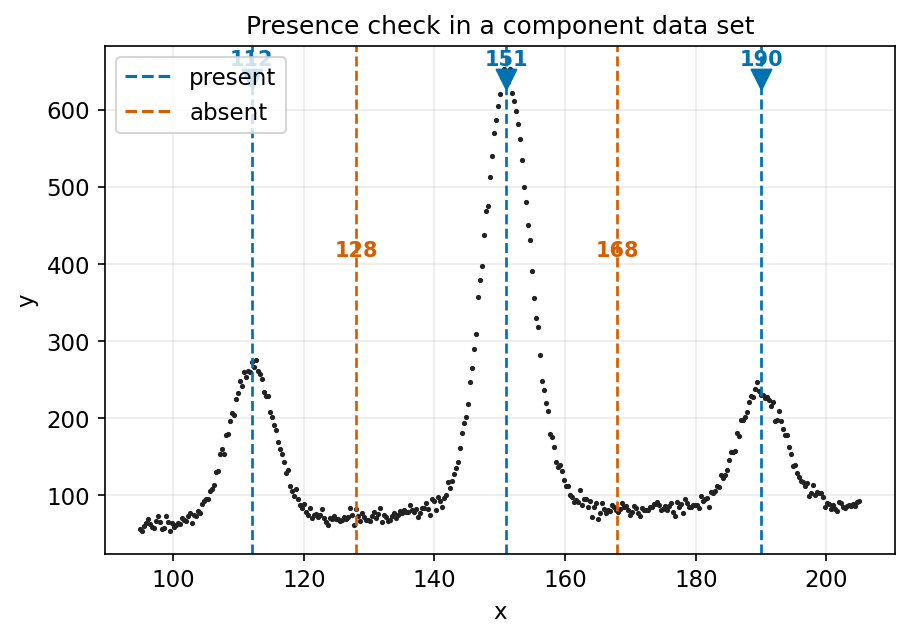
\includegraphics[width=0.82\linewidth]{figures/fig_presence.png}
\caption{Presence check: present peaks green, absent red; dashed lines mark the
reference positions.}
\end{figure}

% =====================================================================
\section{Graphical interface}
\code{PeakCheckGUI} embeds a Matplotlib~\citep{Hunter2007} plot in a Tkinter
window. The automatic search provides the starting point; the user keeps control
by mouse. A fourth control row exposes the baseline method (Section~5) and the
optional position refinement (Section~14), so both are reachable from the GUI as
well as the TOML. The central click handler:

\codehdr{peakcheck/gui.py --- PeakCheckGUI.\_on\_click() (add/remove peaks by mouse)}
\begin{lstlisting}[style=py]
def _on_click(self, event):
    if self.x is None or event.inaxes != self.ax or event.xdata is None:
        return
    idx = int(np.argmin(np.abs(self.x - event.xdata)))
    if event.button == 1:           # add
        if idx not in self.peaks:
            self.peaks.append(idx)
            self.peaks.sort()
            self._redraw()
    elif event.button == 3:         # remove nearest
        if self.peaks:
            clicked_x = self.x[idx]
            peak_xs = self.x[self.peaks]
            nearest = self.peaks[int(np.argmin(np.abs(peak_xs - clicked_x)))]
            if abs(self.x[nearest] - clicked_x) < (self.x[-1] - self.x[0]) * 0.04:
                self.peaks.remove(nearest)
                self._redraw()
\end{lstlisting}
\begin{itemize}
\item \code{np.argmin(np.abs(self.x - event.xdata))} finds the data point nearest
the click.
\item Left click (\code{button == 1}) adds that index as a peak (if not already
present).
\item Right click (\code{button == 3}) removes the nearest existing peak, provided
it is close enough (within $4\,\%$ of the $x$ span).
\item \code{_redraw()} updates markers and labels immediately.
\end{itemize}

\begin{figure}[h]
\centering
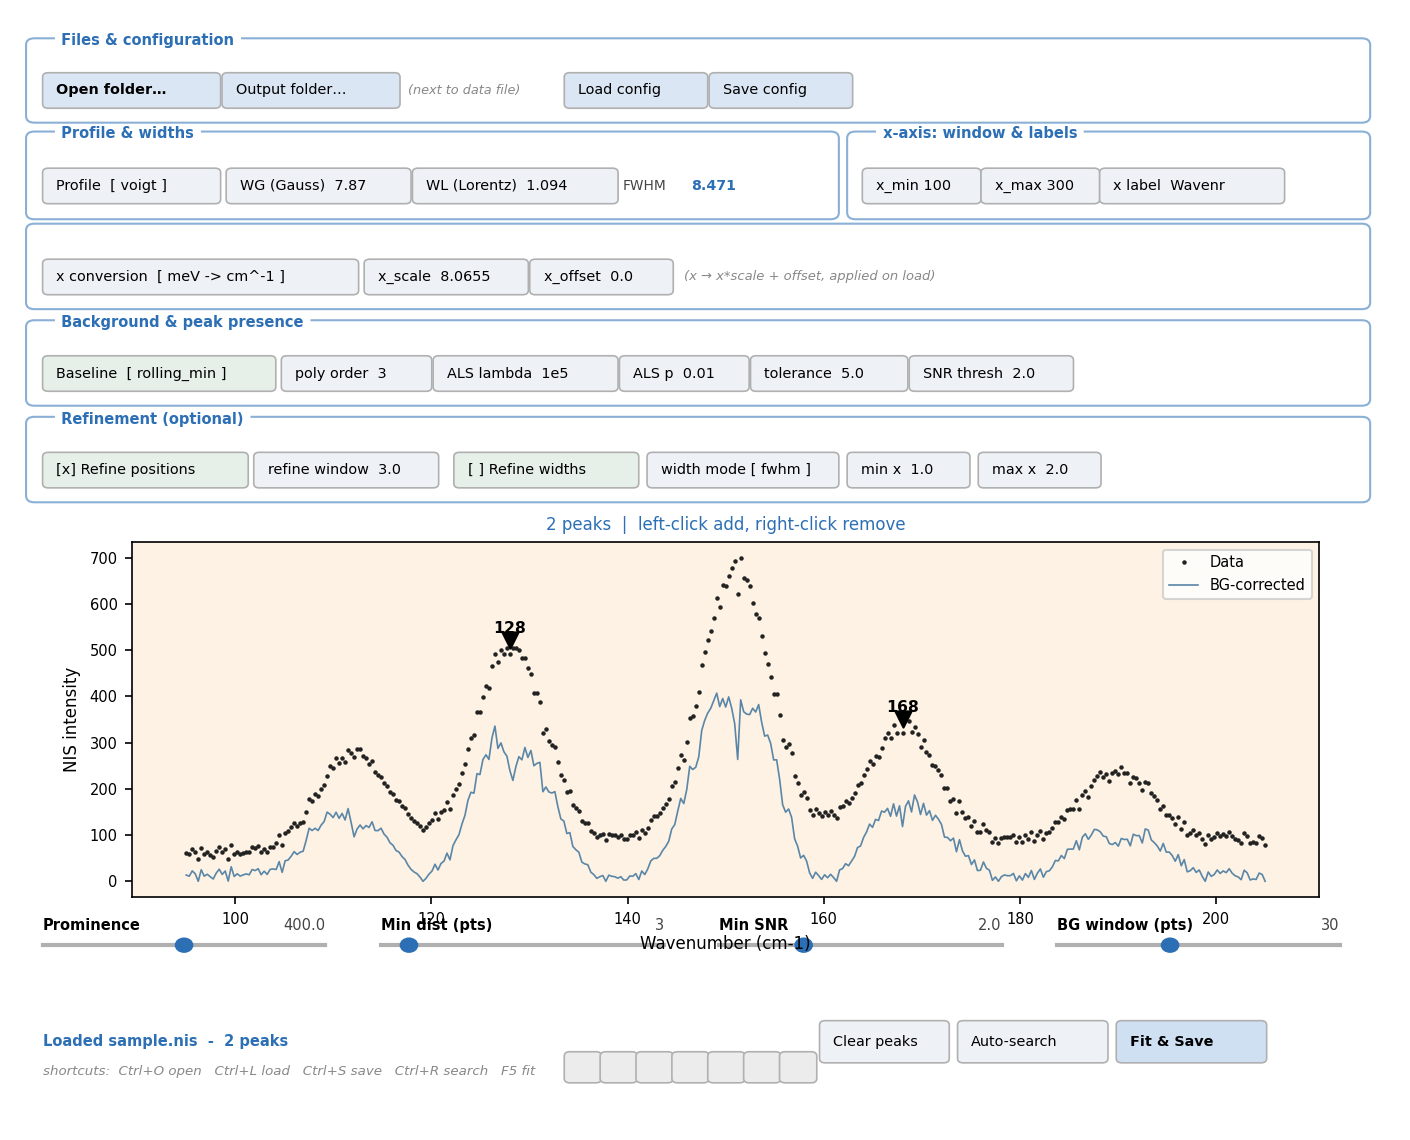
\includegraphics[width=0.92\linewidth]{figures/fig_gui.png}
\caption{The PeakCheck window: control bars, plot with peak markers, sliders and
toolbar.}
\end{figure}

% =====================================================================
\section{Outputs and reproducibility}
\code{save_excel()} writes up to six sheets; \code{save_csv()} writes the same
data as a single plain 7-bit ASCII file \code{*_results.csv} (enforced by
\code{_ascii()}) with five labelled sections. Both carry the full parameter block
from \code{gather_parameters()} as a header.

\begin{table}[h]\small\centering
\begin{tabularx}{\linewidth}{@{}l L@{}}
\toprule
\textbf{Sheet} & \textbf{Content}\\
\midrule
\code{Intensities} & peak, NNLS amplitude, standard error, measured intensity per component\\
\code{Positions}   & reference and measured positions (tracks shifts)\\
\code{Presence}    & binary matrix $1$ (green) / $0$ (red) --- the key result\\
\code{Fit_Data}    & raw data, errors, corrected, sum and individual components\\
\code{Components_Raw} & each component's raw $(x, y, \text{error})$ as side-by-side blocks (only when components are analysed)\\
\code{Parameters}  & full run metadata (path, profile, widths, window, error mode, $\chi^2$/$R^2$, versions)\\
\bottomrule
\end{tabularx}
\end{table}
Every run is thus fully documented and reconstructable from its config (or the
CSV header) alone.

\subsection{Presence matrix with colour coding}
The \code{Presence} sheet writes a $1$ (green) or $0$ (red) per peak and component
and colours the cell accordingly, so the key result is readable at a glance:

\codehdr{peakcheck/output.py --- save\_excel(), Presence sheet}
\begin{lstlisting}[style=py]
FOUND_FILL    = PatternFill("solid", start_color="C6EFCE")    # green
NOTFOUND_FILL = PatternFill("solid", start_color="FFC7CE")    # red
# ... for each (peak, component) cell:
c = ws3.cell(row=i, column=j)
if fmask[idx]:
    c.value, c.fill, c.font = 1, FOUND_FILL, FOUND_FONT
else:
    c.value, c.fill, c.font = 0, NOTFOUND_FILL, NOTFOUND_FONT
\end{lstlisting}

\subsection{Plain ASCII CSV with a parameter header}
The CSV file is deliberately written as 7-bit ASCII (via \code{errors="replace"}
and \code{_ascii()} for the column names) so it reads without encoding issues on
any system and in any pipeline. The single \code{*_results.csv} holds five
labelled sections --- \code{Intensities}, \code{Positions}, \code{Presence},
\code{Fit_Data} and \code{Components_Raw} --- separated by \code{# === SECTION:
<name> ===} lines, and starts with the full parameter block as a commented
header:

\codehdr{peakcheck/output.py --- save\_csv(), ASCII enforcement \& header}
\begin{lstlisting}[style=py]
def _ascii(s):
    return str(s).encode("ascii", "replace").decode("ascii")   # force 7-bit ASCII

# one results file; component column labels are forced to ASCII:
comp_labels = [_ascii(os.path.splitext(os.path.basename(f))[0])
               for f, _, _, _ in component_results]

# the file opens in ASCII mode and starts with the parameter block:
with open(out_path, "w", newline="", encoding="ascii", errors="replace") as fh:
    for ln in _csv_header_lines(params):
        fh.write(ln + "\n")
\end{lstlisting}

\subsection{What the parameter block contains}
\code{gather_parameters()} collects all run metadata into an ordered table ---
input path, axis transform, error provenance, profile and widths, windows,
$\chi^2$/$R^2$ and the versions of numpy/scipy/Python. When width refinement is
enabled it also records the mode, the width bounds and the resulting per-peak
FWHM and scale factors. Every run is thus fully documented:

\codehdr{peakcheck/output.py --- gather\_parameters() (excerpt)}
\begin{lstlisting}[style=py]
p["Reference file"]   = os.path.abspath(cfg.reference_file)
p["x transform"]      = f"x*{cfg.x_scale} + {cfg.x_offset}"
p["Errors from file"] = "yes" if had_errors else "no (estimated from data)"
p["Profile"]          = str(cfg.profile).lower()
p[f"Effective FWHM{unit}"] = round(cfg.effective_fwhm(), 4)
p["chi2_reduced"]     = round(stats["chi2_red"], 4)
p["R2"]               = round(stats["r2"], 6)
p["numpy"]  = np.__version__
p["scipy"]  = scipy.__version__
p["Python"] = sys.version.split()[0]
\end{lstlisting}
This block goes into both the Excel \code{Parameters} sheet and the header of
every CSV file. Together with the saved TOML configuration, a run is therefore
fully reproducible.

% =====================================================================
\section{Worked example}
The bundled example (\code{example_data/}) shows the complete workflow on
synthetic NIS data~\citep{Sturhahn1995,Sturhahn2004,ScheidtDurbinSage2005}. The reference \code{sample.nis} contains
five peaks; the $x$ values are stored in meV. The configuration
\code{nis_example.toml} selects \code{x_conversion = "meV -> cm^-1"}, so the whole
analysis runs in $\mathrm{cm}^{-1}$.

\textbf{1. Read \& transform.} The meV axis (about $11.8$--$25.4$~meV) is mapped by
the factor $8.065544$ into the range $95$--$205~\mathrm{cm}^{-1}$.

\textbf{2. Fit.} With fixed positions $[112, 128, 151, 168, 190]~\mathrm{cm}^{-1}$
and the instrumental widths ($\code{wg}=7.87$, $\code{wl}=1.09$), the weighted
NNLS fit returns the integrated intensities:

\begin{table}[h]\small\centering
\begin{tabular}{@{}lccccc@{}}
\toprule
Peak ($\mathrm{cm}^{-1}$) & 112 & 128 & 151 & 168 & 190\\
\midrule
Amplitude $A_k$ & 1969 & 4111 & 5675 & 2408 & 1507\\
\bottomrule
\end{tabular}
\end{table}

The fit quality is $\chi^2_\nu = 5.5$ at $R^2 = 0.945$. The elevated $\chi^2_\nu$
is intentional and instructive here: the data carry genuine Poisson errors, so any
model simplification (one fixed width for all peaks) shows up as a systematic
contribution to the reduced chi-square --- exactly the situation of Section~8 in
which \code{statistical} is the correct error mode.

\textbf{3. Presence.} In the component \code{sample_A.nis} the peaks at $128$ and
$168~\mathrm{cm}^{-1}$ are absent by construction. The check on the
background-corrected signal separates them clearly (threshold
\code{snr_thresh}${}=5$):

\begin{table}[h]\small\centering
\begin{tabular}{@{}lccc@{}}
\toprule
Peak ($\mathrm{cm}^{-1}$) & $y_{\text{corr}}$ & $\mathrm{SNR}_{\text{corr}}$ & Result\\
\midrule
112 & 227.6 & 13.8 & present (1)\\
128 & 17.4  & 4.4  & absent (0)\\
151 & 490.5 & 18.9 & present (1)\\
168 & 14.3  & 3.8  & absent (0)\\
190 & 143.8 & 11.4 & present (1)\\
\bottomrule
\end{tabular}
\end{table}

The background-corrected signal separates by more than an order of magnitude
(present ${\sim}140$--$490$ vs absent ${\sim}15$), whereas the raw signal would be
more similar at the same positions because of the background --- the choice of
signal justified in Section~9 makes the decision robust. The presence matrix in
the Excel sheet accordingly reads $A = [1, 0, 1, 0, 1]$.

% =====================================================================
\section{Numerical validation and exactness}
Several of the claims above can be checked directly against reference
implementations and against the bundled example.

\paragraph{The profile is the true Voigt.} Evaluated on a wide grid, PeakCheck's
\code{voigt()} agrees with \code{scipy.special.voigt_profile} to floating-point
precision: the maximum absolute deviation is about $3\times10^{-17}$ and the
maximum relative deviation about $1\times10^{-14}$. The two are therefore
identical up to rounding --- confirming that the profile is the exact convolution
and not a pseudo-Voigt, whose deviation from the true shape is percent-level
(Figures~\ref{fig:voigttrue} and~\ref{fig:conv}).

\paragraph{Area normalisation.} Each profile integrates analytically to one. A
finite-range numerical integral approaches one as the range grows; because the
Lorentzian wings decay only as $1/x^2$, a modest window leaves a few percent of
the area in the tails, which is why the fit window is widened by $3(f_G+f_L)$
(Section~7.1) so that the dominant part of every profile is inside it.

\paragraph{Uniqueness of the amplitude fit.} The weighted NNLS objective
$\lVert W(B\mathbf{A}-\mathbf{y}_\text{corr})\rVert_2^2$ is a convex quadratic
(its Hessian $B^\top W^2 B$ is positive semidefinite) on the convex feasible set
$\mathbf{A}\ge 0$, so the minimiser is unique whenever the active profile columns
are linearly independent. The active-set method of Lawson \&
Hanson~\citep{LawsonHanson1995} reaches it in finitely many steps, and the
solution satisfies the Karush--Kuhn--Tucker conditions: an active peak
($A_k>0$) has a vanishing gradient component, a pinned peak ($A_k=0$) a
non-negative one. A peak that the data do not support therefore receives exactly
$A_k=0$ rather than a noisy small or negative value.

\paragraph{Determinism and reproducibility.} The computational core contains no
random component, so a given configuration --- equivalently, the parameter block
stored in the Excel \code{Parameters} sheet or the CSV header --- reproduces the
result on the same platform. The bundled example doubles as a regression check:
with the shipped \code{nis_example.toml} the fit returns the amplitudes,
$\chi^2_\nu$, $R^2$ and presence matrix quoted in Section~12, and the test suite
asserts the core numerics.

\subsection{Monte-Carlo recovery and error calibration}
The covariance estimate of Section~16 can be checked directly. Injecting the
five amplitudes of the worked example into the noiseless model, adding
independent Gaussian noise with the per-point $\sigma_i$, and re-running the
NNLS fit $N=600$ times yields the recovered amplitudes of
Figure~\ref{fig:mc}. The mean recovered amplitudes coincide with the injected
values --- the largest bias is $0.06\,\sigma$, i.e.\ the estimator is unbiased
to within Monte-Carlo error --- and the empirical scatter (the standard
deviation across the $N$ trials) reproduces the analytic
$\sigma=\sqrt{(B^{\top}W^2B)^{-1}_{kk}}$ to within $6\,\%$ for every peak. The
linear fit therefore returns both the correct amplitudes and a quantitatively
trustworthy error budget whenever the model and the noise estimate are correct.

\begin{figure}[h]\centering
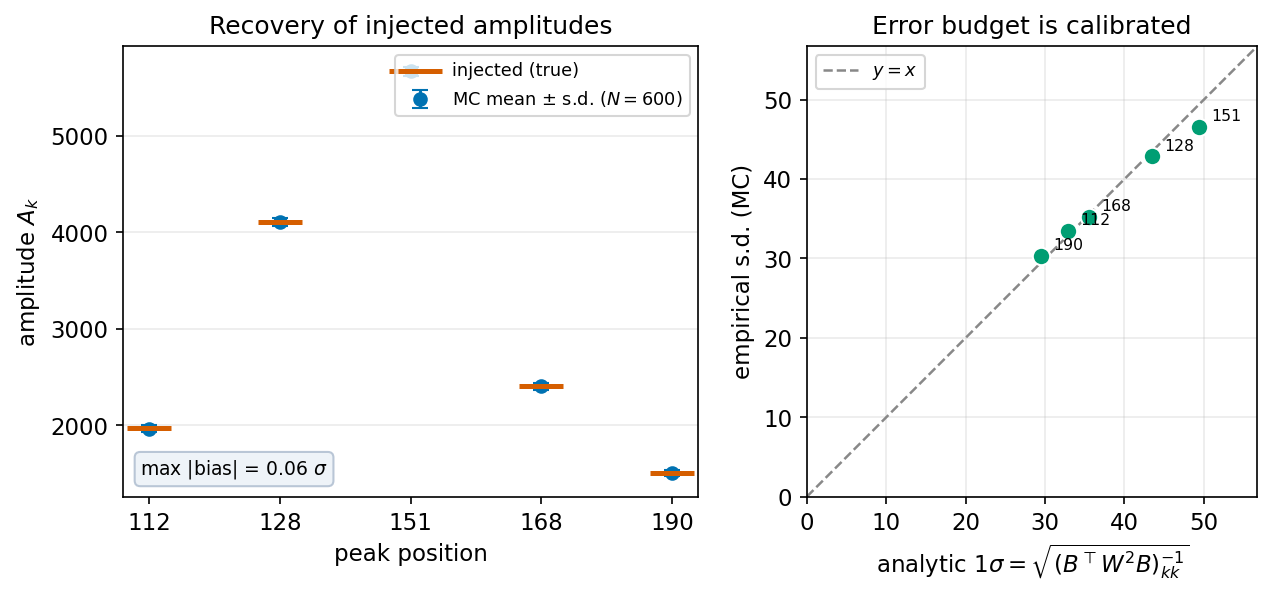
\includegraphics[width=0.96\linewidth]{figures/fig_mc.png}
\caption{Monte-Carlo recovery over $N=600$ noise realisations. Left: the mean
recovered amplitudes (points, with $\pm$ one empirical standard deviation) sit
on the injected values (ticks); the maximum bias is $0.06\,\sigma$. Right: the
empirical scatter versus the analytic $1\sigma$ from the covariance lies on the
$y=x$ line, confirming that the reported errors are calibrated.}
\label{fig:mc}
\end{figure}

% =====================================================================
\section{Assumptions, limitations and parameter selection}
PeakCheck is intentionally a focused tool; knowing what it does \emph{not} do is
part of using it correctly.

\begin{itemize}
\item \textbf{Fixed positions and widths.} The fit is linear --- and hence fast,
unique and robust --- precisely because the peak positions and the two widths are
held fixed. PeakCheck quantifies intensities at known or expected positions; it
does not refine positions or per-peak widths \emph{by default}. An optional
refinement (\code{refine = true}) relaxes this for the positions only: holding
the widths fixed, it refines the centres by a bounded variable-projection fit
(Section~15), each centre constrained to a small window so it cannot migrate
onto a neighbour. If the instrumental resolution is
misestimated or peaks overlap strongly, the fixed-width model absorbs the
mismatch into the amplitudes and into an elevated $\chi^2_\nu$ (Section~8).
\item \textbf{One global noise scale.} Without an error column, a single $\sigma$
is estimated from the high-frequency differences (Section~3). This suits roughly
homoscedastic noise; for strongly count-dependent (Poisson) data spanning orders
of magnitude, supply a genuine error column so the weights $1/\sigma_i$ and the
reported errors are correct.
\item \textbf{Rolling-minimum background.} The baseline model is parameter-light
and robust to peak shape, but it assumes the background varies more slowly than a
peak. A window narrower than a peak eats into it; a window wider than the
background curvature leaves a residual slope (Figure~\ref{fig:bgwin}).
\item \textbf{Presence is a detection, not a fit.} The presence check decides only
whether a peak is present in a component within the tolerance window; it does not
re-fit the component. Its multi-stage logic is deliberately conservative (true
maxima, then clear shoulders, with geometric duplicate resolution).
\end{itemize}

\noindent The handful of parameters that matter most, and how to choose them:

\begin{table}[h]\small\centering
\begin{tabularx}{\linewidth}{@{}l L@{}}
\toprule
\textbf{Parameter} & \textbf{Effect and how to choose}\\
\midrule
\code{bg_window}        & baseline window: wider than a peak FWHM (in points), narrower than the background curvature; $0$ disables it\\
\code{prominence_init}  & search sensitivity: raise to reject noise, lower to catch weak peaks; tune live in the GUI\\
\code{distance_init}    & minimum peak separation in points: $\approx$ the smallest spacing you expect to resolve\\
\code{min_snr_init} / \code{snr_thresh} & SNR gates for search / presence: $2$--$3$ for clean data, $4$--$6$ for noisy spectra\\
\code{tolerance}        & presence window: larger than expected centroid shifts, smaller than the peak spacing\\
\code{error_mode}       & \code{statistical} for genuine $1\sigma$ errors; \code{scaled} for relative weights of unknown scale (Section~8)\\
\bottomrule
\end{tabularx}
\end{table}

\begin{figure}[h]
\centering
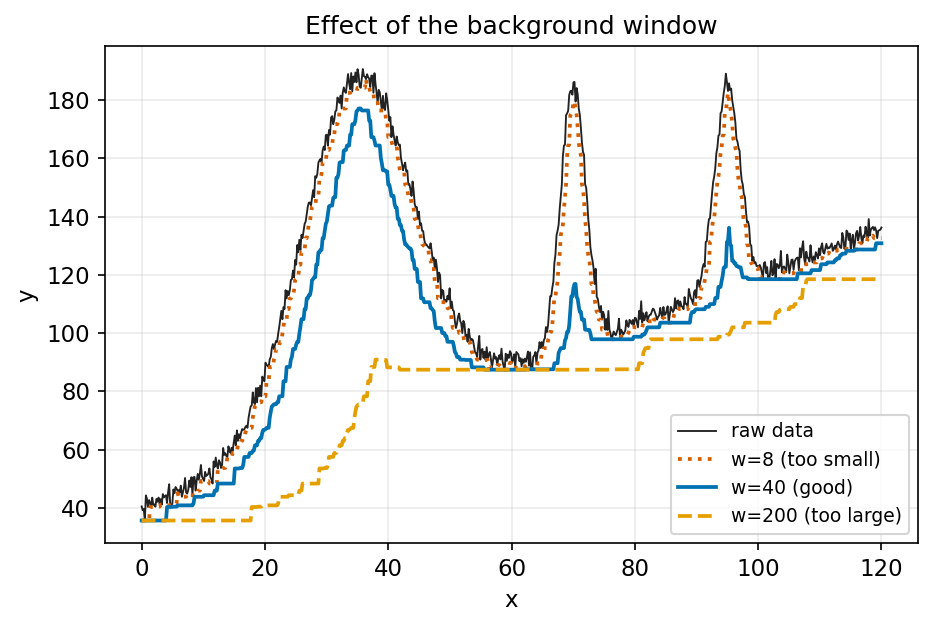
\includegraphics[width=0.74\linewidth]{figures/fig_bg_window.png}
\caption{Choosing the background window. A window much narrower than a peak
follows the peak flanks and is subtracted away (too small); a window much wider
than the baseline curvature cannot track the slope and leaves a residual ramp
(too large). A window a few times the peak width tracks the baseline while
leaving the peaks intact.}
\label{fig:bgwin}
\end{figure}

% =====================================================================
\section{Relation to nonlinear least-squares fitting}
PeakCheck's central design choice --- fixing the peak positions and the two
widths and fitting only the amplitudes by NNLS --- is what separates it from
general nonlinear peak fitting (Levenberg--Marquardt as in
\code{scipy.optimize.curve_fit}~\citep{SciPyCurveFit}, or \code{lmfit}), which
refines positions and widths as well.

\begin{itemize}
\item \textbf{Convexity and uniqueness.} With positions and widths fixed the
residual is linear in $\mathbf{A}$, the objective is convex, and NNLS returns the
unique global optimum --- no starting values, no local minima, no convergence
failures. A nonlinear fit over positions/widths is non-convex
(Figure~\ref{fig:land}): it needs good initial guesses and can settle in a local
minimum.
\item \textbf{Non-negativity.} NNLS enforces $A_k\ge 0$ exactly, so an absent mode
gets $A_k=0$. A nonlinear solver returns whatever minimises the residual,
including unphysical negative areas, unless explicitly bounded.
\item \textbf{Speed.} One NNLS solve replaces an iterative sequence of Jacobian
evaluations (Section~17).
\item \textbf{What is given up.} PeakCheck does \emph{not} refine positions or
widths; it assumes the instrumental resolution (the two widths) is known and the
positions are given or picked in the GUI. When those are themselves unknown or
variable, a full nonlinear fit is the right tool; an elevated $\chi^2_\nu$
(Section~8) is the signal that the fixed-shape assumption is being strained.
\end{itemize}

\begin{figure}[h]
\centering
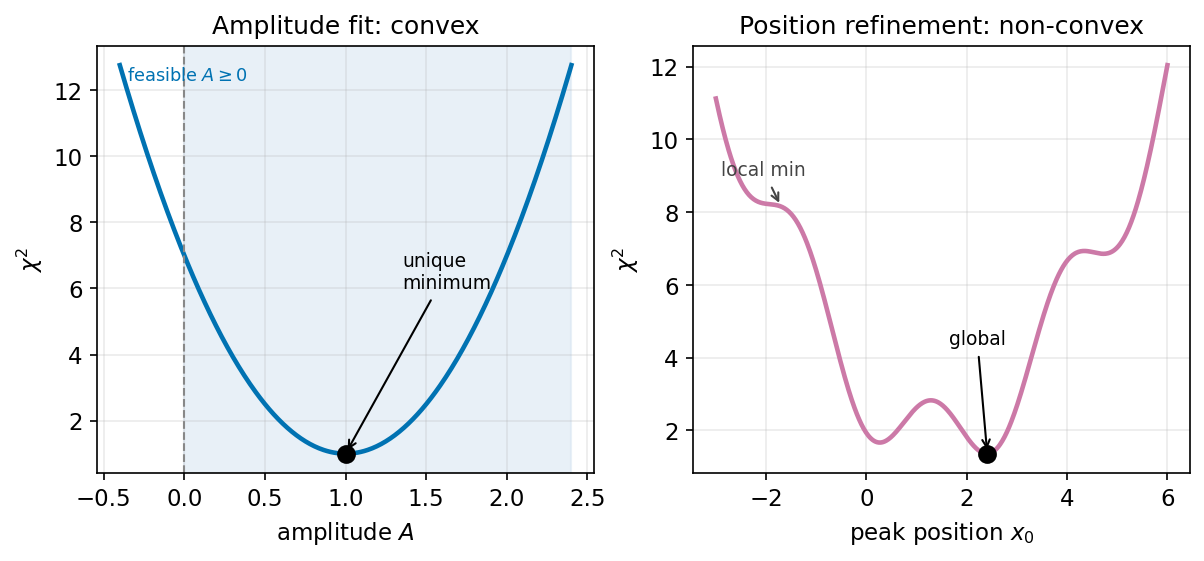
\includegraphics[width=0.92\linewidth]{figures/fig_landscape.png}
\caption{Why fixing the shape helps. Left: with positions and widths fixed the
objective is convex in the amplitude, so there is a single minimum on the
feasible region $A\ge 0$. Right: refining a peak position makes the objective
non-convex, with local minima a solver can fall into.}
\label{fig:land}
\end{figure}

\begin{table}[h]\small\centering
\begin{tabularx}{\linewidth}{@{}l L L@{}}
\toprule
 & \textbf{PeakCheck (fixed-shape NNLS)} & \textbf{general nonlinear fit}\\
\midrule
free parameters   & amplitudes only                   & positions, widths, amplitudes\\
objective         & convex --- unique optimum         & non-convex --- local minima\\
initial guess     & none needed                       & required, sensitive\\
non-negativity    & guaranteed                        & only if bounded\\
positions/widths  & fixed (assumed known)             & refined\\
typical use       & intensity quantification at known modes & full line-shape characterisation\\
\bottomrule
\end{tabularx}
\caption{When the modes and the resolution are known, the fixed-shape NNLS fit is
more robust and reproducible; when they are not, a nonlinear fit is appropriate.}
\end{table}

\paragraph{A middle ground.} The optional position refinement (\code{refine},
Section~14) is a deliberately small step in the nonlinear direction: the
amplitudes are still obtained by NNLS through variable projection, only the
centres are refined, and only within a bounded window. It recovers
slightly-offset positions without surrendering the non-negativity and
robustness of the linear fit, but it does not replace a full line-shape
analysis when the widths themselves are unknown. Figure~\ref{fig:refine}
illustrates the effect.

\begin{figure}[h]\centering
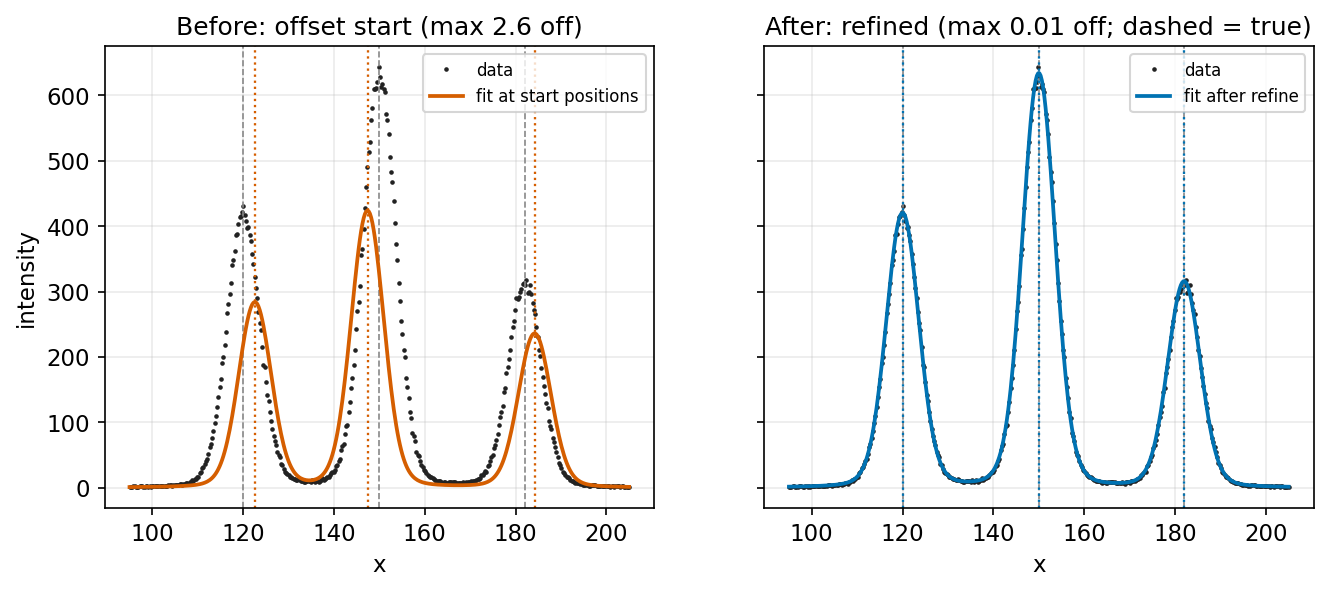
\includegraphics[width=0.96\linewidth]{figures/fig_refine.png}
\caption{The optional position refinement. Left: with deliberately offset start
centres (dotted) the fixed-position fit is visibly misaligned with the true
centres (dashed grey). Right: with \code{refine = true} the bounded
variable-projection step recovers the centres to a small fraction of a sample
spacing, while the amplitudes remain non-negative throughout.}
\label{fig:refine}
\end{figure}

\paragraph{Per-peak widths.} The same variable-projection idea extends to the
widths. With \code{refine\_widths = true} one width \emph{scale} per peak is
introduced and refined by the same bounded least-squares solve, the amplitudes
again obtained by NNLS for every trial set of widths. \code{width\_mode} selects
whether the whole Voigt is scaled (\code{"fwhm"}: both $\sigma$ and $\gamma$, so
the effective FWHM scales with the factor --- the Olivero--Longbothum width is
homogeneous of degree one in $(f_G,f_L)$) or only the Gaussian part
(\code{"sigma"}: inhomogeneous broadening, the Lorentzian lifetime width fixed).
Each scale is constrained to
$[\texttt{width\_min\_factor},\texttt{width\_max\_factor}]$ times the
instrumental width, with the lower bound defaulting to the instrument itself so a
band can never be reported narrower than the resolution. Because every refined
width is an extra free parameter, the degrees of freedom are reduced accordingly
(\code{n\_extra\_params} in \code{fit\_statistics}), so $\chi^2_\nu$ is computed
honestly; even so, freeing widths \emph{always} lowers $\chi^2_\nu$, and for
overlapping or weak peaks width and amplitude (or a neighbour's intensity) trade
off, which is exactly why the bounds matter. Figure~\ref{fig:widths} shows the
recovery on a genuinely broadened peak.

\begin{figure}[h]\centering
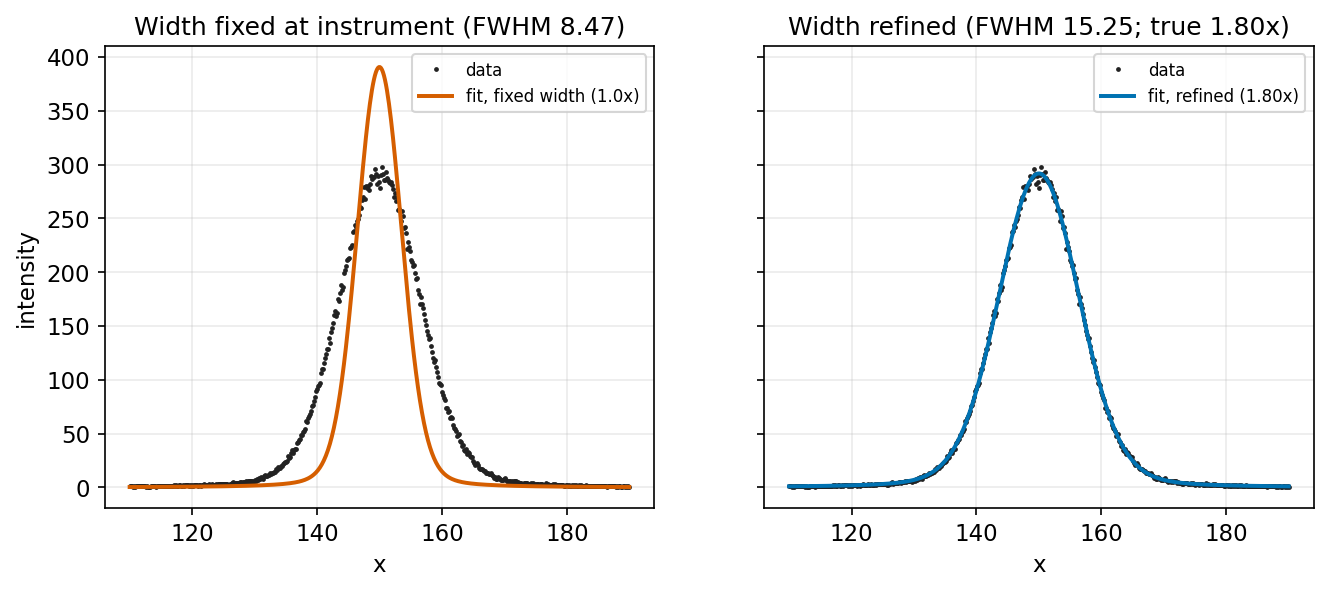
\includegraphics[width=0.96\linewidth]{figures/fig_widths.png}
\caption{Optional per-peak width refinement. Left: with the width fixed at the
instrumental resolution the fit undershoots a peak that is genuinely broader.
Right: with \code{refine\_widths = true} the bounded variable-projection step
recovers the per-peak width (here close to the true broadening factor) while the
amplitude stays non-negative.}
\label{fig:widths}
\end{figure}

% =====================================================================
\section{Error budget: a worked covariance example}
The per-amplitude uncertainties are the square roots of the diagonal of the
linear covariance matrix. For the active peaks ($A_k>0$) with weighted design
matrix $B_\text{act}$ and $W=\operatorname{diag}(1/\sigma_i)$,
\[
C = \big(B_\text{act}^{\top} W^2 B_\text{act}\big)^{-1},
\qquad
\sigma_{A,k} = \sqrt{C_{kk}},
\qquad
\rho_{ij} = \frac{C_{ij}}{\sqrt{C_{ii}\,C_{jj}}},
\]
and in \code{scaled} mode each $\sigma_{A,k}$ is multiplied by $\sqrt{\chi^2_\nu}$
(Section~8). The off-diagonal correlations $\rho_{ij}$ quantify how much two
amplitudes trade off against each other: strongly overlapping peaks are
anticorrelated (raising one can be partly absorbed by lowering its neighbour),
whereas well-separated peaks are nearly independent.

For the bundled example (Section~12, \code{statistical} mode) the fitted
amplitudes and their $1\sigma$ errors are
$1969\pm33$, $4111\pm45$, $5675\pm52$, $2408\pm36$ and $1507\pm27$.
Figure~\ref{fig:errcorr} shows the amplitudes with these error bars and the
corresponding correlation matrix. Because the peaks here are well separated, the
off-diagonal correlations are small ($|\rho|\lesssim 0.05$) and the amplitudes
are effectively independent --- the diagonal errors can be read off directly. For
closely spaced modes the same matrix would show pronounced anticorrelations, a
warning that the individual amplitudes are less well determined than their
diagonal errors alone suggest. Statistical mode corresponds to
\code{curve_fit(..., absolute_sigma=True)} and scaled mode to
\code{absolute_sigma=False}.

\begin{figure}[h]
\centering
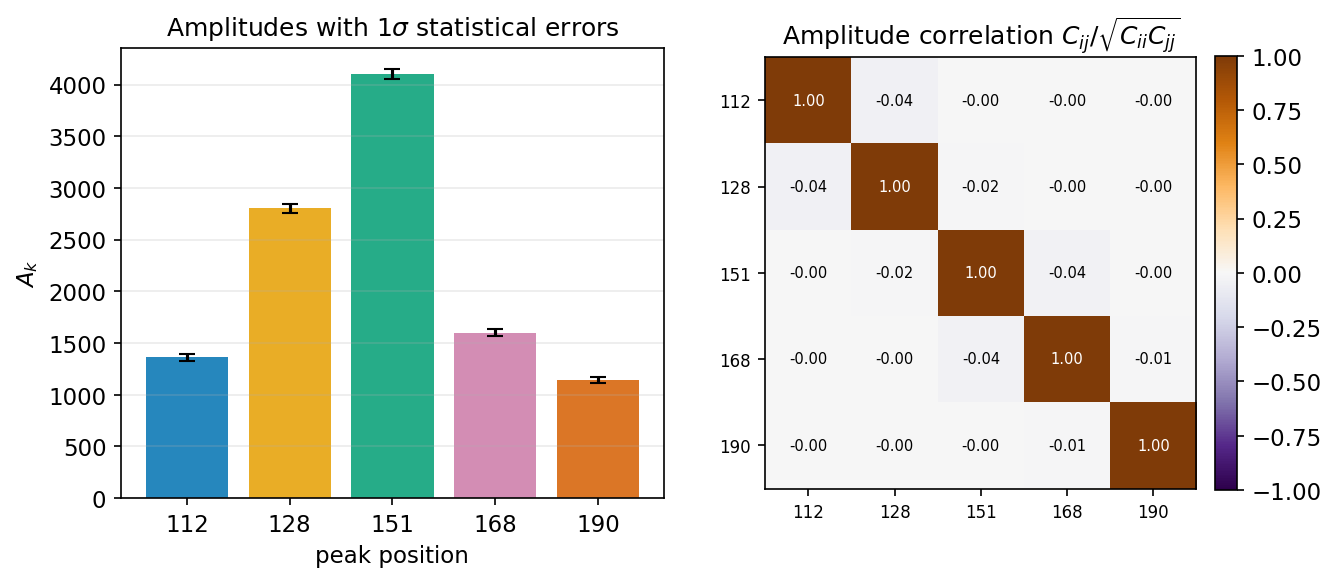
\includegraphics[width=0.96\linewidth]{figures/fig_error_corr.png}
\caption{Left: fitted amplitudes with $1\sigma$ statistical errors from
$\sqrt{C_{kk}}$. Right: the amplitude correlation matrix
$\rho_{ij}=C_{ij}/\sqrt{C_{ii}C_{jj}}$ for a representative five-peak spectrum;
the small off-diagonal values reflect the well-separated peaks.}
\label{fig:errcorr}
\end{figure}

% =====================================================================
\section{Computational complexity and performance}
The pipeline is linear in the spectrum length and modest in the number of peaks.
Building the design matrix $B$ costs $O(N K)$ profile evaluations ($N$ points,
$K$ peaks; each a Faddeeva call). Forming the weighted normal equations is
$O(N K^2)$, and the active-set NNLS solve then works on the small $K\times K$
system, with $K$ typically a few to a few tens. The peak search
(\code{find_peaks}) and the rolling-minimum background are $O(N)$. Memory is
$O(N K)$ for $B$, negligible at spectroscopic sizes.

Figure~\ref{fig:scaling} confirms this with measured timings: the end-to-end fit
(build $B$ + solve) grows linearly with $N$ from a few hundred to $5\times10^4$
points, and even at the largest size it takes only tens of milliseconds; the NNLS
solve itself stays well below a millisecond, since it sees only the $K$ columns.
Re-fitting on every GUI slider change is therefore effectively instantaneous, and
the dominant cost in practice is file I/O and plotting rather than the numerics.

\begin{figure}[h]
\centering
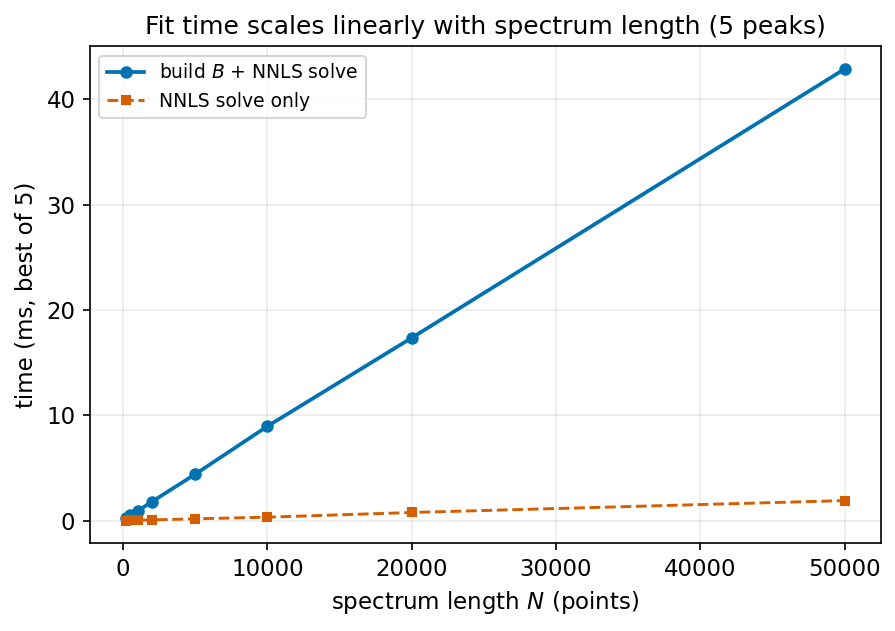
\includegraphics[width=0.78\linewidth]{figures/fig_scaling.png}
\caption{Measured fit time versus spectrum length (five peaks, best of five
runs). Building $B$ and solving the NNLS together scale linearly with $N$; the
NNLS solve itself is sub-millisecond because it only sees the $K$ profile
columns.}
\label{fig:scaling}
\end{figure}

% =====================================================================
\section{Parameter reference}
All \code{Config} parameters with their meaning (in TOML-section order):

\begin{table}[h]\small\centering
\begin{tabularx}{\linewidth}{@{}l L@{}}
\toprule
\textbf{Parameter} & \textbf{Meaning}\\
\midrule
\code{reference_file} & data set in which the peaks are defined\\
\code{component_glob} & component search pattern; empty $=$ \code{<name>_*}\\
\code{error_column}   & \code{"auto"} / \code{"none"} / column index\\
\code{fio_x_column}, \code{fio_y_column} & FIO only: x/y column by name or 1-based index (default y \code{"nisp"})\\
\code{x_conversion}   & named preset (e.g.\ \code{"meV -> cm^-1"})\\
\code{x_transform}    & \code{"affine"} or \code{"reciprocal"}\\
\code{x_scale}, \code{x_offset} & factor/offset or numerator of the transform\\
\code{x_label}, \code{y_label}, \code{x_unit} & axis labels and x-axis unit string (display only)\\
\code{profile}        & \code{"voigt"} / \code{"gauss"} / \code{"lorentz"}\\
\code{wg}, \code{wl}  & Gaussian and Lorentzian FWHM\\
\code{x_min}, \code{x_max} & search range (target unit); empty $=$ full range\\
\code{bg_window}      & background window size (points); $0=$ off\\
\code{baseline_method} & \code{"rolling_min"} / \code{"polynomial"} / \code{"als"}\\
\code{baseline_poly_order} & order of the polynomial baseline\\
\code{baseline_als_lambda}, \code{baseline_als_p} & ALS smoothness and asymmetry\\
\code{prominence_init}, \code{distance_init}, \code{min_snr_init} & starting values of the automatic search\\
\code{refine}, \code{refine_window} & refine positions (bounded); max shift in x-units\\
\code{refine_widths}, \code{width_mode} & refine per-peak widths; \code{"fwhm"} or \code{"sigma"}\\
\code{width_min_factor}, \code{width_max_factor} & width bounds as factors of the instrumental width\\
\code{tolerance}      & $\pm$ window of the presence check (target unit)\\
\code{snr_thresh}     & SNR threshold of the presence check\\
\code{presence_baseline_corrected} & SNR on corrected (true) or raw (false) signal\\
\code{error_mode}     & \code{"statistical"} or \code{"scaled"}\\
\code{output_dir}     & target folder for outputs; empty $=$ next to the reference file\\
\code{write_csv}, \code{write_excel} & write the CSV / Excel outputs (both default \code{true})\\
\code{plot_dpi}       & resolution (dpi) of the saved plots\\
\code{peaks}          & optional fixed peak positions (otherwise search/mouse)\\
\bottomrule
\end{tabularx}
\end{table}

Since TOML has no \code{null}, empty fields are turned into \code{None} on load by
\code{_coerce_nullable()}:

\codehdr{peakcheck/config.py --- \_coerce\_nullable() (empty strings to None)}
\begin{lstlisting}[style=py]
def _coerce_nullable(cfg: Config) -> None:
    for key in ("x_min", "x_max"):
        v = getattr(cfg, key)
        if v == "" or v is None:
            setattr(cfg, key, None)
        else:
            setattr(cfg, key, float(v))
\end{lstlisting}

% =====================================================================
\section{References}
\renewcommand{\refname}{}
\vspace{-2.2em}
\bibliographystyle{plainnat}
\bibliography{references}

% =====================================================================
\section{Notation}
\begin{table}[h]\small\centering
\begin{tabularx}{\linewidth}{@{}l L@{}}
\toprule
\textbf{Symbol} & \textbf{Meaning}\\
\midrule
$x,\ x_0$ & abscissa (working units) and peak centre\\
$\sigma$ & Gaussian standard deviation\\
$\gamma$ & Lorentzian half width at half maximum\\
$f_G = 2\sqrt{2\ln 2}\,\sigma$ & Gaussian FWHM (\code{wg})\\
$f_L = 2\gamma$ & Lorentzian FWHM (\code{wl})\\
$f_V$ & total Voigt FWHM (Olivero--Longbothum)\\
$G,\ L,\ V$ & Gaussian, Lorentzian, Voigt profiles (each of unit area)\\
$w(z) = e^{-z^2}\operatorname{erfc}(-iz)$ & Faddeeva function (\code{scipy.special.wofz})\\
$z = \dfrac{(x-x_0)+i\gamma}{\sigma\sqrt 2}$ & complex argument of $w$\\
$P_k$ & area-normalised profile of peak $k$\\
$B,\ B_{ik}=P_k(x_i)$ & profile (design) matrix\\
$A_k$ & fitted amplitude $=$ integrated intensity of peak $k$\\
$W=\operatorname{diag}(1/\sigma_i)$ & diagonal weight matrix\\
$\sigma_i$ & per-point $1\sigma$ uncertainty\\
$\mathbf{y},\ \mathbf{y}_\text{corr}$ & raw and background-corrected intensities\\
$r_i$ & residual (corrected data minus model)\\
$N,\ N_\text{active}$ & points in the fit window; peaks with $A_k>0$\\
$N_\text{extra}$ & extra free parameters (refined positions/widths; $0$ by default)\\
$\chi^2,\ \chi^2_\nu$ & chi-square and reduced $\chi^2 = \chi^2/(N-N_\text{active}-N_\text{extra})$\\
$R^2$ & coefficient of determination\\
$\eta$ & pseudo-Voigt mixing fraction (shown for contrast; not used by PeakCheck)\\
\bottomrule
\end{tabularx}
\end{table}

\bigskip
\noindent\rule{\linewidth}{0.4pt}\\[2pt]
{\footnotesize PeakCheck \textperiodcentered\ Technical Supplement \textperiodcentered\
\textcopyright\ 2026 Lukas Knauer, RPTU Kaiserslautern-Landau, AG Sch\"unemann
\textperiodcentered\ MIT license. The code excerpts are reproduced from the
modules of the \code{peakcheck} package (with brief inline comments and, where
marked by \code{...}, abbreviations); the figures were produced with the routines
contained in the program.}

\end{document}
